\documentclass[conference]{IEEEtran}

% ---------- Math / Figures ----------
\usepackage{amsmath,amssymb,amsfonts,amsthm}
\usepackage{graphicx}
\graphicspath{{figures/}{./}}
\usepackage{booktabs}
\usepackage{multirow}
\usepackage{placeins}
\usepackage{threeparttable}
\usepackage{tabularx}
\usepackage{array}
\usepackage{enumerate}
\usepackage{siunitx}


% ---------- Symbols ----------
\usepackage{pifont}
\newcommand{\cmark}{\ding{51}}  % ✓
\newcommand{\xmark}{\ding{55}}  % ✗
\newcolumntype{Y}{>{\raggedright\arraybackslash}X}

% ---------- Text / Utils ----------
\usepackage{times}
\DeclareFontShape{OT1}{ptm}{m}{scit}{<->ssub * ptm/m/sc}{}
\emergencystretch=3em
\hfuzz=500pt
\hbadness=10000
\vbadness=10000
\setcounter{bottomnumber}{2}
\setcounter{totalnumber}{4}
\renewcommand{\bottomfraction}{0.95}
\renewcommand{\textfraction}{0.05}
\usepackage{soul}
\usepackage{url}
\usepackage{xcolor}
%\usepackage[switch]{lineno}  % removed for submission
\usepackage{xr}

\theoremstyle{definition}
\newtheorem{definition}{Definition}
\newtheorem{challenge}{Challenge}
% ---------- Biblatex (IMPORTANT) ----------
% 建议加 csquotes；biblatex 在某些环境下会提示它
\usepackage{csquotes}
\usepackage[
  backend=biber,
  style=ieee,
  citestyle=numeric-comp,
  sorting=none,
  sortcites=true,
  doi=false,
  url=false
]{biblatex}

\addbibresource{reference.bib}
\renewcommand*{\bibfont}{\fontsize{8}{9.6}\selectfont}

% ---------- Hyperref should be near the end ----------
\usepackage[hidelinks]{hyperref}
\hypersetup{pdfauthor={}}
\theoremstyle{plain}
\newtheorem{theorem}{Theorem}
\newtheorem{lemma}{Lemma}
\newtheorem{corollary}{Corollary}
\newtheorem{proposition}{Proposition}
% *** CITATION PACKAGES ***
%
%\usepackage{cite}
% cite.sty was written by Donald Arseneau
% V1.6 and later of IEEEtran pre-defines the format of the cite.sty package
% \cite{} output to follow that of the IEEE. Loading the cite package will
% result in citation numbers being automatically sorted and properly
% "compressed/ranged". e.g., [1], [9], [2], [7], [5], [6] without using
% cite.sty will become [1], [2], [5]--[7], [9] using cite.sty. cite.sty's
% \cite will automatically add leading space, if needed. Use cite.sty's
% noadjust option (cite.sty V3.8 and later) if you want to turn this off
% such as if a citation ever needs to be enclosed in parenthesis.
% cite.sty is already installed on most LaTeX systems. Be sure and use
% version 5.0 (2009-03-20) and later if using hyperref.sty.
% The latest version can be obtained at:
% http://www.ctan.org/pkg/cite
% The documentation is contained in the cite.sty file itself.






% *** GRAPHICS RELATED PACKAGES ***
%
\ifCLASSINFOpdf
  % \usepackage[pdftex]{graphicx}
  % declare the path(s) where your graphic files are
  % \graphicspath{{../pdf/}{../jpeg/}}
  % and their extensions so you won't have to specify these with
  % every instance of \includegraphics
  % \DeclareGraphicsExtensions{.pdf,.jpeg,.png}
\else
  % or other class option (dvipsone, dvipdf, if not using dvips). graphicx
  % will default to the driver specified in the system graphics.cfg if no
  % driver is specified.
  % \usepackage[dvips]{graphicx}
  % declare the path(s) where your graphic files are
  % \graphicspath{{../eps/}}
  % and their extensions so you won't have to specify these with
  % every instance of \includegraphics
  % \DeclareGraphicsExtensions{.eps}
\fi
% graphicx was written by David Carlisle and Sebastian Rahtz. It is
% required if you want graphics, photos, etc. graphicx.sty is already
% installed on most LaTeX systems. The latest version and documentation
% can be obtained at:
% http://www.ctan.org/pkg/graphicx
% Another good source of documentation is "Using Imported Graphics in
% LaTeX2e" by Keith Reckdahl which can be found at:
% http://www.ctan.org/pkg/epslatex
%
% latex, and pdflatex in dvi mode, support graphics in encapsulated
% postscript (.eps) format. pdflatex in pdf mode supports graphics
% in .pdf, .jpeg, .png and .mps (metapost) formats. Users should ensure
% that all non-photo figures use a vector format (.eps, .pdf, .mps) and
% not a bitmapped formats (.jpeg, .png). The IEEE frowns on bitmapped formats
% which can result in "jaggedy"/blurry rendering of lines and letters as
% well as large increases in file sizes.
%
% You can find documentation about the pdfTeX application at:
% http://www.tug.org/applications/pdftex


 \pagestyle{plain}



% *** FLOAT PACKAGES ***
%
%\usepackage{fixltx2e}
% fixltx2e, the successor to the earlier fix2col.sty, was written by
% Frank Mittelbach and David Carlisle. This package corrects a few problems
% in the LaTeX2e kernel, the most notable of which is that in current
% LaTeX2e releases, the ordering of single and double column floats is not
% guaranteed to be preserved. Thus, an unpatched LaTeX2e can allow a
% single column figure to be placed prior to an earlier double column
% figure.
% Be aware that LaTeX2e kernels dated 2015 and later have fixltx2e.sty's
% corrections already built into the system in which case a warning will
% be issued if an attempt is made to load fixltx2e.sty as it is no longer
% needed.
% The latest version and documentation can be found at:
% http://www.ctan.org/pkg/fixltx2e


%\usepackage{stfloats}
% stfloats.sty was written by Sigitas Tolusis. This package gives LaTeX2e
% the ability to do double column floats at the bottom of the page as well
% as the top. (e.g., "\begin{figure*}[!b]" is not normally possible in
% LaTeX2e). It also provides a command:
%\fnbelowfloat
% to enable the placement of footnotes below bottom floats (the standard
% LaTeX2e kernel puts them above bottom floats). This is an invasive package
% which rewrites many portions of the LaTeX2e float routines. It may not work
% with other packages that modify the LaTeX2e float routines. The latest
% version and documentation can be obtained at:
% http://www.ctan.org/pkg/stfloats
% Do not use the stfloats baselinefloat ability as the IEEE does not allow
% \baselineskip to stretch. Authors submitting work to the IEEE should note
% that the IEEE rarely uses double column equations and that authors should try
% to avoid such use. Do not be tempted to use the cuted.sty or midfloat.sty
% packages (also by Sigitas Tolusis) as the IEEE does not format its papers in
% such ways.
% Do not attempt to use stfloats with fixltx2e as they are incompatible.
% Instead, use Morten Hogholm'a dblfloatfix which combines the features
% of both fixltx2e and stfloats:
%
% \usepackage{dblfloatfix}
% The latest version can be found at:
% http://www.ctan.org/pkg/dblfloatfix




% *** PDF, URL AND HYPERLINK PACKAGES ***
%
%\usepackage{url}
% url.sty was written by Donald Arseneau. It provides better support for
% handling and breaking URLs. url.sty is already installed on most LaTeX
% systems. The latest version and documentation can be obtained at:
% http://www.ctan.org/pkg/url
% Basically, \url{my_url_here}.




% *** Do not adjust lengths that control margins, column widths, etc. ***
% *** Do not use packages that alter fonts (such as pslatex).         ***
% There should be no need to do such things with IEEEtran.cls V1.6 and later.
% (Unless specifically asked to do so by the journal or conference you plan
% to submit to, of course. )


% correct bad hyphenation here
\hyphenation{op-tical net-works semi-conduc-tor}


\begin{document}
%
% paper title
% Titles are generally capitalized except for words such as a, an, and, as,
% at, but, by, for, in, nor, of, on, or, the, to and up, which are usually
% not capitalized unless they are the first or last word of the title.
% Linebreaks \\ can be used within to get better formatting as desired.
% Do not put math or special symbols in the title.
\title{TSIP for Proof-Carrying Trajectory Integrity in Private Location Aggregation}


% author names and affiliations
% use a multiple column layout for up to three different
% affiliations
\author{\IEEEauthorblockN{Anonymous Authors}
	\IEEEauthorblockA{Submitted for Double-Blind Review}}


% use for special paper notices
%\IEEEspecialpapernotice{(Invited Paper)}


\IEEEoverridecommandlockouts
\makeatletter\def\@IEEEpubidpullup{6.5\baselineskip}\makeatother
\IEEEpubid{\parbox{\columnwidth}{
		Network and Distributed System Security (NDSS) Symposium 2027\\
		22 - 26 March 2027, Seoul, Republic of Korea\\
  ISBN 979-8-9919276-8-0\\
  https://dx.doi.org/10.14722/yyy.2027.230400\\
		www.ndss-symposium.org
}
\hspace{\columnsep}\makebox[\columnwidth]{}}


% make the title area
\maketitle

% As a general rule, do not put math, special symbols or citations
% in the abstract
\begin{abstract}
Privacy-preserving location aggregation publishes useful heatmaps from mobile
trajectories without exposing raw coordinates. Existing protocols validate each
report in isolation. They cannot detect when individually well-formed reports
collectively describe a physically impossible path.
We present \textsc{TSIP} (\underline{T}emporal-\underline{S}patial
\underline{I}ntegrity \underline{P}roof), a proof-carrying integrity layer for
Encode-Shuffle-Analyze (ESA)-style aggregation. Each submission carries a
128\,B Groth16 proof. The proof links the hidden location to the prior accepted
state under speed and Anchor-Distance Window Continuity (ADWC) bounds. It also
derives the primary heatmap cell from the hidden coordinate and binds that cell
to the submitted payload. This in-circuit binding closes a gap left by
compositions of prior verifiable aggregation and ZK-validity systems. A client
cannot prove a plausible trajectory for one cell while contributing shares
bound to another.
Raw coordinates remain hidden under salted commitments, AEAD-routed shares, and
non-colluding aggregation. We evaluate \textsc{TSIP} on T-Drive and GeoLife with
1{,}000 clients. The 3{,}056-constraint circuit rejects teleportation,
credential-theft impersonation, replay, proof-payload substitution, and
boundary-violating drift with zero false rejects on benign traces. A native
verifier sustains 3{,}320\,proofs/s on 16 cores and supports about 199\,K
concurrent clients within a 60\,s window. We characterize the residual
in-envelope attack surface and show that deployment-layer controls reduce its
heatmap effect below benign noise.
\end{abstract}

\begin{IEEEkeywords}
location aggregation, trajectory integrity, zero-knowledge proofs,
differential privacy, secure aggregation
\end{IEEEkeywords}



\section{Introduction}
\label{sec:intro}

Location heatmaps derived from mobile trajectories are a basic tool in
urban computing. Traffic engineering, public transit planning, and
environmental sensing all rely on population-level spatial statistics,
while raw user coordinates must remain hidden from the infrastructure
~\cite{Zheng2010GeoLife,Yuan2010Tdrive}. Existing privacy-preserving
location analytics systems therefore combine local differential privacy
(LDP)~\cite{Dwork2006calibrating,Andres2013geoi}, shuffle-style
analytics~\cite{Bittau2017Prochlo,Cheu2019distributed}, and secure
aggregation~\cite{Shamsabadi2025Nebula,Segal2017PracticalSecAgg}.
These mechanisms reduce disclosure risk and improve the privacy-utility
trade-off of released heatmaps, but they validate privacy rather than
physical plausibility: an accepted report can still be inconsistent with any
realistic trajectory.

Recent incidents show that trajectory integrity remains a live operational
problem rather than a legacy concern. Strava reported removing millions of
anomalous activities from segment leaderboards over the past year, including
vehicle-recorded activities, wrong sport uploads, and corrupted GPS
traces~\cite{strava-leaderboard-integrity-2026}. In a 2025 ride-hailing
fraud case, attackers used virtual location software to complete implausible
orders and maliciously extend route distance and duration to obtain platform
fees and subsidies~\cite{cctv-ridehailing-virtual-location-2025}. Although
these platforms are not themselves private MCS aggregation systems, they expose
the same structural weakness: validating location reports independently does
not prevent an adversary from constructing a fabricated trajectory across
time. Short zero-knowledge proofs can enforce per-report predicates, such as
whether an encoded cell index lies in range~\cite{Chowdhury2022EIFFeL}, yet
privacy and single-round validity do not imply cross-round consistency.
Neither differential privacy, which is intentionally agnostic to input
plausibility, nor existing verifiable aggregation, which checks stateless
predicates, closes this gap.

The missing property is \emph{cross-round trajectory integrity}. Accepted
reports from the same client should remain consistent with a private,
physically bounded trajectory and with the payload that is ultimately admitted
into aggregation. \textsc{TSIP} is not a proof of ground-truth physical
presence. Our threat model instead targets coordinated malicious clients
against honest-but-curious, non-colluding servers, and asks a narrower systems
question: can the infrastructure reject post-enrollment reports that are
inconsistent with a committed private trajectory envelope, without learning
the trajectory itself? The full model appears in \S\ref{sec:threat}.

The required motion relation seems simple: displacement should not exceed
$v_{\max}\!\cdot\!\Delta t$. Enforcing it inside private aggregation is less
simple. The verifier must check motion without learning either endpoint. The
relation must be stateful to prevent replay. The admitted report must be bound
to the same hidden cell for which motion validity is proved. Finally, local
step validity is insufficient by itself: a sequence of locally plausible steps
can still drift beyond a configured $K$-round envelope. These requirements
must hold simultaneously.

A natural design is to combine EIFFeL-style ZK norm proofs, VDAF validity
checks, and off-circuit trajectory filtering. This composition is insufficient.
The proof can certify one hidden cell while the admitted shares encode another
payload cell, and an off-circuit filter cannot enforce the same hidden state
relation without exposing trajectory information. This proof-payload gap is
the basis of attack A6. We make it explicit in \S\ref{sec:circuit} and close
it inside the circuit via C21 (Table~\ref{tab:ablation}).

\textsc{TSIP} closes the gap by making the proof-payload link an in-circuit
relation. The Groth16 statement derives the hidden primary cell from the
hidden coordinate and binds that primary to the report payload and A/R
share-content commitments under the current report context. Each client
maintains a commitment chain. Each submission carries a compact
\textsc{TSIPMain} proof that links the current location to the previous
accepted state under per-step and ADWC constraints. The Shuffler verifies
\textsc{TSIPMain}, chain continuity, and transport integrity before forwarding
to secure aggregation. The downstream $\varepsilon$-DP release is
unchanged~\cite{Corrigan2017Prio,Balle2019privacy}. This design trades
per-report unlinkability for cross-round integrity. The Shuffler observes
chain topology and timing as protocol-control leakage rather than public-output
DP, while coordinates and primary cells remain hidden under salted
commitments, ZK, AEAD-routed shares, and non-colluding aggregation.

To summarize, our contributions are:
\begin{itemize}
\item We formalize \emph{cross-round trajectory integrity} for ESA-style
private location aggregation and introduce the \emph{Anchor-Distance Window
Continuity} (ADWC) predicate, which couples per-step speed bounds with
$K$-round drift bounds.

\item We design and implement \textsc{TSIP}, a stateful proof-carrying
integrity layer for private heatmap aggregation. \textsc{TSIP} binds hidden
motion validity, ADWC window continuity, chain continuity, and same-primary
payload consistency inside the aggregation proof, preventing proof-payload
substitution attacks.

\item We evaluate \textsc{TSIP} on T-Drive and GeoLife with up to $1{,}000$
clients. In the recommended $K=6$ profile, \textsc{TSIP} rejects all modeled
out-of-envelope and proof-payload substitution attacks with zero
circuit-level false rejects on the evaluated benign traces. Combined with a
lightweight behavioral external layer, \textsc{TSIP} reduces false hotspot
promotion to zero in the evaluated settings across $\rho\in[0.01,0.30]$
(Figure~\ref{fig:hotspot-pollution}).
\end{itemize}
\section{Related Work}
\label{sec:related-work}

\textsc{TSIP} relates to three lines of work. These lines are
privacy-preserving location aggregation, verifiable secure aggregation, and
location integrity. Table~\ref{tab:positioning} positions \textsc{TSIP}
against representative prior systems.

\begin{table*}[t]
\centering
\caption{Positioning of \textsc{TSIP} against representative prior systems,
highlighting the unique combination of cross-round continuity, windowed
envelope enforcement, and hidden primary share binding that prior systems leave
to separate layers.
A filled mark (\cmark) indicates native support, a partial mark ($\circ$)
indicates partial or deployment layer coverage, and a dash (\xmark) indicates no
coverage.}
\label{tab:positioning}
\footnotesize
\setlength{\tabcolsep}{2pt}
\renewcommand{\arraystretch}{1.05}
\begin{tabularx}{\textwidth}{@{}>{\raggedright\arraybackslash}p{2.35cm} >{\raggedright\arraybackslash}p{1.55cm} >{\centering\arraybackslash}p{1.15cm} c c c >{\centering\arraybackslash}p{1.05cm} >{\centering\arraybackslash}p{1.35cm} Y@{}}
\toprule
\textbf{System} & \textbf{Target} &
\shortstack{\textbf{DP}\\\textbf{release}} &
\shortstack{\textbf{Per-round}\\\textbf{integrity}} &
\shortstack{\textbf{Cross-round}\\\textbf{continuity}} &
\shortstack{\textbf{Post-enroll.}\\\textbf{traj. envelope}} &
\shortstack{\textbf{A2b}\\\textbf{coverage}} &
\shortstack{\textbf{Proof}\\\textbf{size}} &
\textbf{Notes} \\
\midrule
Prio~\cite{Corrigan2017Prio}                   & aggregate stats     & out-of-scope & \cmark    & \xmark     & \xmark & \xmark & \mbox{\(\sim\)\,\SI{1}{KB}} & SNIP range checks \\
Prochlo~\cite{Bittau2017Prochlo}               & shuffle analytics   & \cmark       & \xmark    & \xmark     & \xmark & \xmark & --                    & ESA paradigm \\
Nebula~\cite{Shamsabadi2025Nebula}             & histograms          & \cmark       & \xmark    & \xmark     & \xmark & \xmark & --                    & shuffle-model histograms \\
Pure LDP / RAPPOR~\cite{Erlingsson2014RAPPOR}  & aggregate stats     & \cmark       & \xmark    & \xmark     & \xmark & \xmark & --                    & local randomization \\
EIFFeL~\cite{Chowdhury2022EIFFeL}              & FL updates          & $\circ$      & \cmark    & \xmark     & \xmark & \xmark & \mbox{\(\sim\)\,\SI{100}{KB}}\textsuperscript{$\ddagger$} & norm-bound ZK \\
VDAF + EIFFeL strawman                        & private telemetry   & \cmark       & \cmark    & \xmark     & \xmark & \xmark & \mbox{\(\gtrsim\)\,\SI{100}{KB}} & measurement-local validity only, no hidden predecessor/anchor relation \\
Geo-Ind.~\cite{Andres2013geoi}                 & location queries    & $\circ$      & \xmark    & \xmark     & \xmark & \xmark & --                    & metric DP, not heatmap aggregation \\
\midrule
\textbf{\textsc{TSIP}}                         & location heatmaps   & \cmark (pure $\varepsilon$) & \cmark & \cmark & \cmark & $\circ$ & \SI{128}{B} & hidden-primary binding with external A2b controls \\
\bottomrule
\end{tabularx}
\vspace{2pt}
{\footnotesize $^\ddagger$EIFFeL size scales with gradient dimension $d$.}
\end{table*}

\subsection{Privacy-Preserving Location Aggregation}

Differential privacy and location-privacy mechanisms protect released
statistics or query answers but do not validate physical
plausibility~\cite{Dwork2006calibrating,Dwork2014algorithmic,Andres2013geoi,Shokri2011Quantifying,Primault2019Survey}.
Foundational DP results~\cite{Dwork2006calibrating,Warner1965Randomized,Kairouz2021Advances}
and variants including R\'enyi DP~\cite{Mironov2017Renyi}, Gaussian
DP~\cite{Dong2022Gaussian}, and deep-learning DP~\cite{Abadi2016DeepDP}
follow the same input-agnostic principle. Local-DP frequency
estimation~\cite{Erlingsson2014RAPPOR,Wang2017LocalFreq,Bassily2015Local,Wang2019MultidimLDP,Kasiviswanathan2011Local}
and shuffle-model systems~\cite{Bittau2017Prochlo,Shamsabadi2025Nebula,Balle2020PrivateSummation,Ghazi2021Power}
improve the privacy-utility trade-off but do not check trajectory integrity.
Privacy amplification analyses~\cite{Erlingsson2019Amplification,Feldman2021Hiding}
strengthen the release model, but they keep the same input-agnostic stance.
Geo-indistinguishability~\cite{Andres2013geoi,Bordenabe2014OptimalGeo,Chatzikokolakis2013Broadening}
and offline trajectory anonymization~\cite{Sweeney2002kAnon,Terrovitis2008Trajectory,Nergiz2009Towards,Wang2023PrivTrace,Du2023LDPTrace}
address related but different problems. Neither provides online,
per-submission integrity for live aggregation. Human mobility exhibits strong
regularities~\cite{Gonzalez2008Mobility,Song2010Predictability} and individual
uniqueness~\cite{Montjoye2013Unique}, motivating temporal~\cite{Xiao2015Temporal}
and anonymous~\cite{Gruteser2003Anonymous} protections.

\textsc{TSIP} keeps the ESA and DP release layer, but inserts proof-carrying
trajectory-integrity checks before aggregation. Complementary FL systems
address scalability~\cite{Bonawitz2019FLScale,Yang2019FedML} and deployment
challenges~\cite{Li2020FLChallenges} but do not enforce per-client trajectory
consistency. Compared with Prochlo and
Nebula, which target full per-report unlinkability, \textsc{TSIP} operates
under a different privacy model. Per-user chain topology and submission timing
are visible to the Shuffler, while raw coordinate values and primary cells
remain hidden from individual servers. This is an intentional design trade-off,
not an oversight. The leakage is enumerated in \S\ref{sec:threat} and excluded
from the $\varepsilon_{\mathrm{total}}$ accounting.

\subsection{Verifiable Secure Aggregation}

Verifiable aggregation systems check whether client messages satisfy
single-round predicates. Prio uses SNIPs for aggregate statistics and range
checks~\cite{Corrigan2017Prio}. Secure aggregation protocols hide individual
inputs during aggregation~\cite{Segal2017PracticalSecAgg,Bell2020SecureSingle,
Bonawitz2019FLScale,McMahan2017FedAvg}. And EIFFeL adds
zero-knowledge norm-bound proofs for federated-learning updates
~\cite{Chowdhury2022EIFFeL}. Complementary work on Byzantine-robust FL
aggregation~\cite{Blanchard2017Krum,Yin2018Byzantine,Cao2021FLTrust},
FL poisoning attacks and defenses~\cite{Fang2020Poisoning,
Bagdasaryan2020Backdoor,Nguyen2022FLAME}, and FL inference
privacy~\cite{Melis2019Inference} address related integrity and confidentiality
challenges in the FL setting but do not enforce cross-round physical constraints.
ELSA, Camel, and ACORN improve malicious
robustness, shuffle-model aggregation, or input validation in federated
learning settings~\cite{Ma2023ELSA,Xu2024Camel,Bell2023ACORN}. These systems
validate submissions round by round. Their predicates do not express physical
mobility constraints between round $t$ and round $t{+}1$ for the same client.

Recent Verifiable Distributed Aggregation Function (VDAF) standardization efforts further systematize multi-server private
aggregation. VDAFs such as Prio3 and Poplar1 allow aggregation servers to
validate encoded measurements while keeping individual measurements hidden when
at least one aggregation server is honest. These protocols are a natural
substrate for private telemetry, but their validity predicates remain
measurement-local. They do not bind one client's current report to its
previously accepted hidden state, window anchor, or trajectory-continuity
policy. \textsc{TSIP} is complementary. It adds a proof-carrying stateful
integrity layer before the aggregation release path, while leaving downstream
private aggregation and DP semantics unchanged. Recent VDAF standardization,
including Prio3 and Poplar1, provides multi-server private aggregation, but
its validity predicates remain measurement-local. Combining VDAF with an
EIFFeL-style proof still leaves the cross-round and payload-binding gap, as
the strawman row in Table~\ref{tab:positioning} makes explicit.

\subsection{Location Integrity and Proof-of-Location}

Proof-of-location and secure-localization systems aim to establish physical
presence or proximity using timed challenge-response, GPS, WiFi, beacons,
trusted hardware, or external witnesses. Such mechanisms address
single-report truthfulness, enrollment trust, or physical presence, often at
the cost of additional infrastructure, interaction, or hardware assumptions.
GPS-spoofing attacks show that claimed coordinates cannot be trusted in
adversarial settings without independent verification
~\cite{Tippenhauer2011GPS}. Continuity-based or mobility-trace analyses can
help detect inconsistent motion patterns
~\cite{Hoh2007Preserving,Shokri2011Quantifying}, while anonymous-credential
mechanisms can bind device identities to enrollment attestations without
revealing them to aggregation servers
~\cite{Rosenberg2023ZKCreds,Rathee2022Zebra}.

\textsc{TSIP} addresses a different layer. It does not claim ground-truth
presence and does not replace proof-of-location at enrollment. Instead, it
enforces consistency among claimed hidden locations after a client has entered
the system. This makes it complementary to proof-of-location, Trusted Execution Environment (TEE)-based
attestation, secure-element sealing, and anonymous-credential mechanisms:
those mechanisms can strengthen enrollment or device-secret protection, while
\textsc{TSIP} enforces private cross-round continuity and proof-payload
binding inside the aggregation pipeline. \textsc{TSIP} uses Groth16~\cite{Groth2016pairing} and ZK-friendly hash functions~\cite{Grassi2021Poseidon,Albrecht2016MiMC} as implementation tools rather than as proof-system contributions. We refer to~\cite{Goldwasser1989ZK,Gabizon2019PLONK,BenSasson2014SNARKs,Parno2013Pinocchio,Setty2020Spartan,Kothapalli2022Nova,Bunz2018Bulletproofs,Wahby2018Doubly,Kate2010KZG,Grassi2022RC,Wen2024ZKCircuit,BenSasson2019Aurora,Sasson2014Zerocash} for related ZK literature.
\section{Preliminaries}
\label{sec:prelim}

This section fixes the notation, cryptographic primitives, attack families,
and security goals used by \textsc{TSIP}. The goals separate three layers that
are easy to conflate. Trajectory-envelope integrity before aggregation,
coordinate and cell confidentiality during verification, and differential
privacy only for the released heatmap. In every aggregation window, each client
maps its private location to a clipped contribution vector
$\tilde{\mathbf{u}}_w^{(i)}\in\mathbb{R}^D$. The vector is one-hot for the
primary visited cell and satisfies $\|\tilde{\mathbf{u}}_w^{(i)}\|_1\le 1$.
The aggregate target is $\mathbf{s}_w=\sum_i\tilde{\mathbf{u}}_w^{(i)}$.
\textsc{TSIP} does not change this target. It only decides which reports may
contribute to it.

\subsection{Differential Privacy}
\label{sec:prelim-dp}

\begin{definition}[Pure Differential Privacy~\cite{Dwork2006calibrating}]
\label{def:dp}
A randomized mechanism $\mathcal{M}:\mathcal{D}\to\mathcal{R}$ satisfies
pure $\varepsilon$-differential privacy if, for all adjacent datasets
$D,D'\in\mathcal{D}$ differing in one user's records and all measurable
$S\subseteq\mathcal{R}$,
\begin{equation}
  \Pr[\mathcal{M}(D)\in S]
  \le e^\varepsilon \Pr[\mathcal{M}(D')\in S].
\end{equation}
\end{definition}

\textsc{TSIP}'s public release provides pure
$\varepsilon_{\mathrm{total}}$-DP under user level adjacency after
per user, per round $L_1$ clipping with sensitivity $\Delta f=1$. The release
layer uses the Sparse Vector Technique (SVT) with Laplace noise. The per-round
budget is
$\varepsilon_{\mathrm{round}}=\varepsilon_{\mathrm{SVT}}+\varepsilon_{\mathrm{val}}$,
and the total budget is
$\varepsilon_{\mathrm{total}}=\sum_{w=1}^T \varepsilon_{\mathrm{round},w}$.
This DP guarantee applies only to the public heatmap output. It does not apply
to protocol-control metadata such as timing, chain topology, mode tags, public
binders, or Shuffler accept/reject outcomes.

\subsection{Zero-Knowledge Proofs and Hash Commitments}
\label{sec:prelim-zk}

\textsc{TSIP} uses Groth16~\cite{Groth2016pairing} over BN254 to prove
trajectory continuity and payload-binding constraints without revealing raw
coordinates or primary heatmap cells. The security analysis relies on Groth16
knowledge soundness and zero-knowledge privacy. The main proof object is denoted
\textsc{TSIPMain}. It includes the trajectory relation, the commitment-chain
relation, ADWC, hidden-cell encoding, and the in-circuit payload-binding
relation.

For in-circuit hashing, \textsc{TSIP} uses Poseidon~\cite{Grassi2021Poseidon}
for salted commitments and MiMC7~\cite{Albrecht2016MiMC} for commitment
chaining. A location commitment is
\begin{equation}
\ell_w=\mathrm{Poseidon}(x_w,y_w,r_w),
\end{equation}
where $r_w$ is a fresh private witness salt with at least 128 bits of entropy.

The payload-binding relation unifies four public binders for the hidden primary,
the report payload, and the two A/R share contents. Their notation is
introduced in \S\ref{sec:system} as
$\mathsf{Com}_{\mathsf{pri}}$, $\mathsf{Com}_{\mathsf{pay}}$,
$\mathsf{Com}_{A}$, and $\mathsf{Com}_{R}$. The circuit enforces that the same
hidden primary derived from the hidden coordinate is the primary used in these
binders.

We use two distinct assumptions for these commitments. For integrity, the
Poseidon and MiMC7 relations are assumed collision-resistant over
$\mathbb{F}_p$, giving binding except with negligible probability. For
privacy, salted Poseidon commitments
$\mathsf{Com}(m,r)=\mathrm{Poseidon}(m,r)$ are modeled as computationally
hiding when $r$ has at least 128 bits of entropy and is not reused. The hiding
assumption is used only in the coordinate-and-cell privacy argument, while
collision resistance is used in the integrity proof.

\subsection{Cross-Round Attack Families}
\label{sec:taxonomy}

The experiments use six concrete attack families A1 to A6. For the security
argument, we group them by the invariant they violate.
Figure~\ref{fig:taxonomy} summarizes the reduction. A1 and A3 violate spatial
continuity. A5 violates Shuffler chain-state continuity. A2a violates secret
binding. A6 violates proof-payload binding. A4 is handled by EA threshold
attestation. A2b is not an in-circuit soundness failure and is treated as
partial coverage in the Discussion.

\begin{figure}[t]
\centering
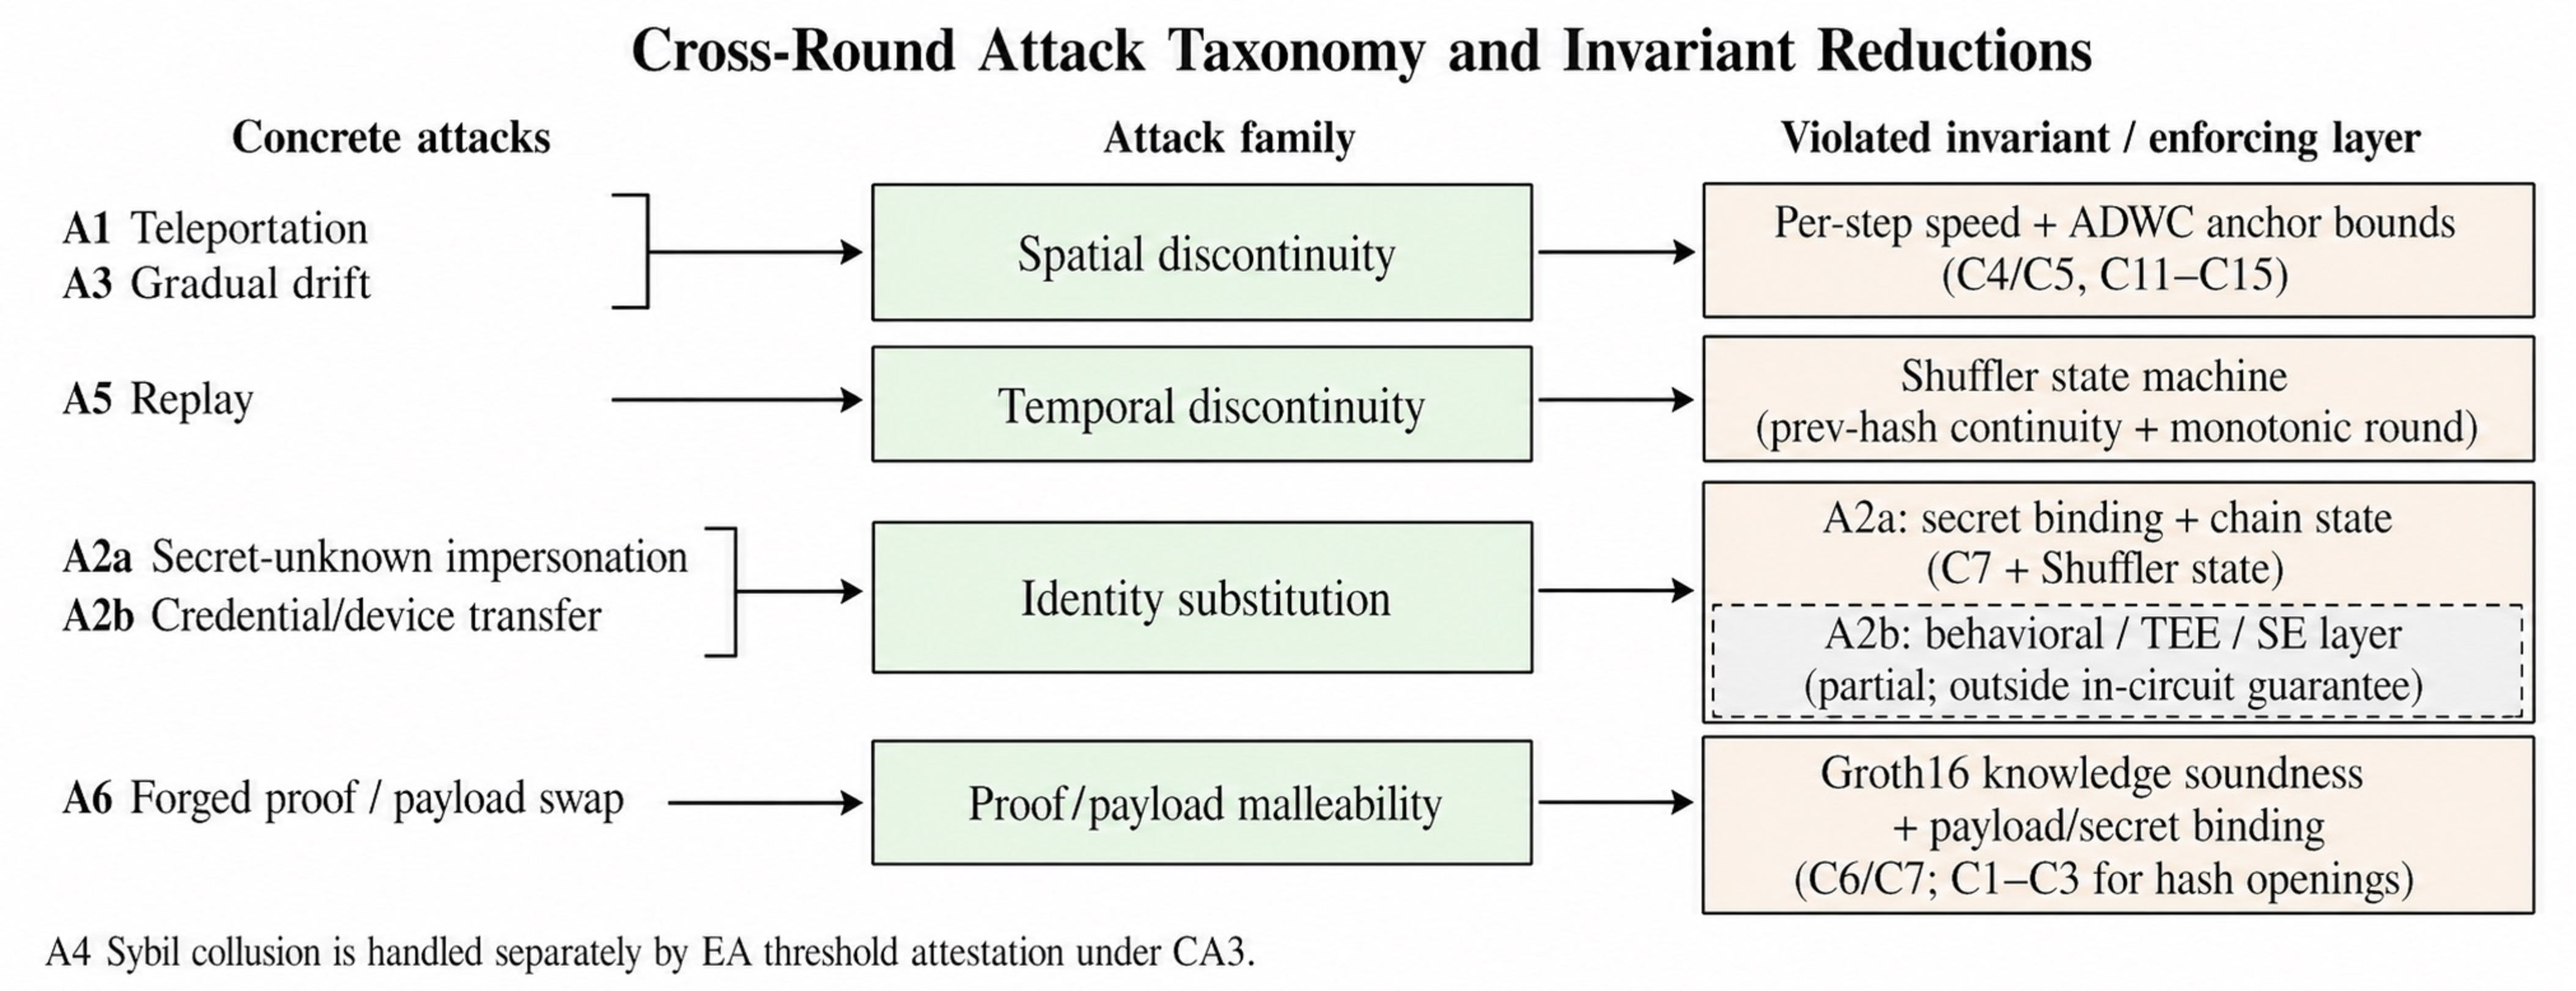
\includegraphics[width=\linewidth]{figures/cross_round_taxonomy.pdf}
\caption{Cross-round attack taxonomy and invariant reductions. Each family
maps to one enforcement layer.}
\label{fig:taxonomy}
\end{figure}

The formal statements appear in \S\ref{sec:security}. Theorem~\ref{thm:traj-integrity}
covers spatial and chain-state invariants. Lemma~\ref{lem:secret-binding}
covers accepted-secret consistency. Theorem~\ref{thm:payload-binding} covers
hidden-primary derivation and payload-binding invariants. Together, these
results cover A1--A6 with negligible error probability.

\subsection{Security and Privacy Goals}
\label{sec:prelim-goals}

\begin{definition}[G1 Post-Enrollment Trajectory Envelope Consistency]
\label{def:g1}
Except with negligible probability, no accepted submission from client $u$
describes a position that violates $u$'s mobility constraints relative to
recently accepted positions. This goal is instantiated by the ADWC predicate
of Definition~\ref{def:adwc}, enforced by C4, C5, and C11 to C15, and linked
across rounds by the Shuffler state machine.
\end{definition}

\begin{definition}[Anchor Distance Window Continuity (ADWC) Predicate]
\label{def:adwc}
For trajectory $\{p_i\}_{i\ge0}$ with $p_i=(x_i,y_i)$, window parameter
$K\ge1$, anchor $a_i=p_{\max(0,i-K)}$, tier speed $\tau_u$, Shuffler-issued
interval $\Delta t_i$, and deployment cap $\mathrm{cap}_{\mathrm{policy}}$,
ADWC holds at step $i$ iff
\begin{equation}
\begin{aligned}
\|p_i-p_{i-1}\|^2 &\le \tau_u^2\Delta t_i^2,\\
\|p_i-a_i\|^2 &\le
\min\bigl(\mathrm{tier\_anchor\_cap}_u^2,
\mathrm{cap}_{\mathrm{policy}}^2\bigr).
\end{aligned}
\end{equation}
For $i<K$, $a_i=p_0$, so warmup uses the same circuit path rather than
skipping anchor checks.
\end{definition}

\begin{definition}[G2 Coordinate-and-Cell Privacy against Honest-but-Curious Servers]
\label{def:g2}
G2 protects both the numeric values of $(x_w,y_w)$ and the derived primary
heatmap cell
$\lfloor x_w/s\rfloor,\lfloor y_w/s\rfloor$. It does not protect
trajectory shape, mobility patterns, or timing metadata observable from chain
topology and accept/reject signals. G2 holds only under the composition
assumptions that Poseidon commitments are hiding, \textsc{TSIPMain}'s Groth16
proof has zero-knowledge privacy, Shuffler-routed ciphertexts satisfy AEAD
confidentiality, the public payload binders reveal no primary index beyond the
stated control metadata, and any one Aggregator's plaintext-share view remains
index hiding without the other Aggregator's share.

Let $\mathcal{A}$ corrupt any server set allowed by \S\ref{sec:threat} and
choose two equal-length candidate trajectory sets $T_0,T_1$ for one honest
user such that both induce the same public metadata, chain topology, timing
metadata, and accept/reject trace. The challenger runs \textsc{TSIP} on
$T_b$ for random $b\in\{0,1\}$ and reveals the joint corrupted-server view
across all rounds. \textsc{TSIP} satisfies G2 if $\mathcal{A}$ distinguishes
$b$ only with negligible advantage. The advantage is bounded by Groth16 zero
knowledge, a constant number of Poseidon hiding hybrids for location and
payload commitments, AEAD confidentiality, and single Aggregator index hiding.
the full statement is Eq.~\eqref{eq:g2-bound} in Appendix~\ref{app:proofs}.
\end{definition}

\noindent\textbf{G3 (Output Privacy).}
As established by Definition~\ref{def:dp} and \S\ref{sec:prelim-dp},
after per-user, per-round $L_1$ clipping the sequence of released heatmaps
satisfies pure $\varepsilon_{\mathrm{total}}$-DP under user-level adjacency.
This goal applies only to the public heatmap release, not to protocol-control
metadata.

\begin{definition}[G4 Enrollment Integrity and Bounded Sybil]
\label{def:g4}
\label{def:g5}
Any accepted enrollment tuple
$(uid,\mathrm{tier\_vmax\_sq},\mathrm{com}_{\mathrm{sec}},
\mathrm{com}_{\mathrm{modeset}})$
must be bound to a valid EA attestation set satisfying the configured
$t$-of-$n$ threshold. Under thresholded EA attestation and non-collusion
assumptions, the number of simultaneously valid Sybil identities is bounded by
the adversary's external budget over per-identity anchor and VC issuance costs.
\end{definition}

G1 captures post enrollment trajectory envelope consistency. G2 captures
confidentiality of hidden coordinates and hidden primary cells during
verification. G3 applies only to the released heatmap. G4 captures
enrollment integrity and Sybil cost. Protocol-control metadata, including
mode\_tag, tier\_vmax\_sq, commitment-chain state, timing, public payload
binders, and Shuffler accept/reject outcomes, is outside the
$\varepsilon_{\mathrm{total}}$ accounting.
\section{System Design}
\label{sec:system}

\textsc{TSIP} follows the Encode-Shuffle-Analyze (ESA) pipeline and inserts a
proof-carrying integrity gate at the Shuffler before forwarding to secure
aggregation. The protocol involves five role types,
Client, Enrollment Attestation Authority (EA), Shuffler, two non-colluding
Aggregators A and R, and Decoder. We close the cross-round and payload-binding
gap left by composing prior verifiable-aggregation and ZK-validity systems
(cf.\ \S\ref{sec:related-work}) inside the main zero-knowledge statement.

\begin{figure*}[!t]
  \centering
  \includegraphics[width=\textwidth]{figures/overview.pdf}
  \caption{
Overview of \textsc{TSIP}. Each client report carries a proof, public binders,
and an encrypted payload package. The Shuffler verifies trajectory continuity,
payload binder consistency, and transport integrity before forwarding only
accepted reports to secure aggregation and downstream DP release.
}
  \label{fig:architecture}
\end{figure*}

\subsection{System Overview}
\label{sec:overview}

Figure~\ref{fig:architecture} shows the full pipeline. Each report first
passes Shuffler-side proof and state verification. Accepted reports then
contribute additive shares to Aggregators A and R, and the Decoder releases
their aggregate as a DP heatmap.

In each reporting round, a client encodes its observation into additive shares
of a clipped one-hot heatmap contribution. The primary cell is derived from the
hidden coordinate. The client updates its commitment chain and generates a
compact \textsc{TSIPMain} proof. The proof binds the current hidden location,
predecessor location, anchor location, identity commitment, tier/mode signals,
hidden primary commitment, report-level payload commitment, and A/R
share-content commitments while proving ADWC with zero-knowledge privacy.

\begin{table}[t]
\centering
\caption{Standard \textsc{TSIP} report workflow with explicit inputs and
outputs.}
\label{tab:protocol-workflow}
\scriptsize
\setlength{\tabcolsep}{3pt}
\begin{tabularx}{\columnwidth}{@{}p{0.9cm}Y@{}}
\toprule
\textbf{Line} & \textbf{Operation} \\
\midrule
Input & User identity, secret state, previous chain state, anchor state,
hidden coordinate, mode tag, timing token, and report context. \\
1 & Derive the hidden primary cell from the current coordinate. \\
2 & Encode the clipped one-hot contribution into two dense shares. \\
3 & Commit to the hidden primary, payload, and A/R share contents. \\
4 & Build the next chain value from the prior state and public binders. \\
5 & Generate \textsc{TSIPMain} over speed, ADWC, identity, and payload-binding
constraints. \\
6 & Verify the proof, timing token, chain continuity, and transport digest at
the Shuffler. \\
7 & Forward only accepted encrypted shares to Aggregators A and R. \\
Output & Accepted aggregate shares and a DP heatmap released by the Decoder. \\
\bottomrule
\end{tabularx}
\end{table}

Additive secret sharing~\cite{Shamir1979Secret} between the two Aggregators
ensures that neither observes plaintext contributions alone. We use
dense/VDAF style fixed-layout shares for single-Aggregator index hiding.
Commitments follow the Pedersen paradigm~\cite{Pedersen1991VSS}, instantiated
with Poseidon over BN254 for ZK-circuit efficiency.

\subsection{Threat Model}
\label{sec:threat}

\noindent\textbf{Adversary capabilities.}
Malicious clients may deviate arbitrarily and may coordinate with one another.
They know all public parameters, including tier speed bounds, ADWC caps, the
window parameter $K$, and the verification key. They do not know honest
clients' device-held secrets or raw coordinates.

\noindent\textbf{Adversary actions.}
The client side attacks considered in this paper are A1 teleportation, A2a
credential theft impersonation, A2b credential/device transfer, A3
gradual drift, A4 Sybil collusion~\cite{Douceur2002Sybil}, A5 replay, and A6 proof-payload
substitution. A1, A2a, A3, A5, and A6 are addressed by the in-circuit
predicate and Shuffler state. A4 relies on EA threshold attestation. A2b and
false enrollment genesis points are deployment-scope issues handled by
external controls rather than by the SNARK relation.

\noindent\textbf{Honest parties and server model.}
Following Prochlo/Nebula's separated role
model~\cite{Bittau2017Prochlo,Shamsabadi2025Nebula} and consistent with
GDPR/CCPA-style multi-operator governance, we assume the Shuffler is honest
but curious. It observes proofs, commitments, ciphertext metadata, and
accept/reject outcomes, but it does not observe plaintext coordinates. We also
assume Aggregators A/R do not collude.

\textbf{Assumption SRV-TS (Server-Issued Timing).}
The Shuffler honestly issues and verifies fresh time slot tokens for each
$(uid,\mathrm{epoch},w)$. Clients cannot choose, replay, or inflate
$\mathrm{step\_dt\_sq}$. They can only prove against a Shuffler issued value.
The token is bound to the user, epoch, round, previous accepted server time,
current coarse server slot, squared interval, and nonce. This avoids relying on
an unpredictable packet receive timestamp during proof generation while still
preventing clients from selecting their own $\Delta t$.

Enrollment authorization follows CA3, at least $t$ out of $n$ enrollment
anchors are non-colluding. The default profile is $t=3,n=5$, and a
single-operator deployment is the degenerate case $t=1,n=1$.

\noindent\textbf{Out of scope and deployment boundaries.}
\textsc{TSIP} does not prove ground-truth enrollment ($c_0$) or prevent
voluntary credential/device transfer (A2b). Production deployments should
combine \textsc{TSIP} with proof-of-location at enrollment, device attestation
or secure-element sealing, and re-enrollment monitoring. These external
controls are not used in Theorems~\ref{thm:traj-integrity}--\ref{thm:payload-binding}.

Crucially, A2b does not create an unrestricted bypass, under \textsc{TSIP}'s
enrollment model, each accepted identity requires thresholded EA attestation
(CA3) and a valid Verifiable Credential (VC) for its tier. Transferring a
credential and device secret to another party therefore degrades to a
Sybil-cost problem, the attacker must still acquire $t$ valid anchor
signatures and a tier VC per identity, and each identity's spatial influence
remains bounded by the public envelope
($\le 34.09\%$ of the grid per $K$-window at $K{=}6$).
Theorem~\ref{thm:bounded-sybil} bounds the number of simultaneously active
Sybil identities under the adversary's external budget. Thus A2b is covered by
the same budget bound argument as Sybil collusion (A4), not by a cryptographic
guarantee inside the SNARK.

Warmup raises the cost of false genesis by requiring $N_{\mathrm{warm}}{=}\max(K,2)$ plausible rounds before aggregation. Collusion of both Aggregators is outside G2's single Aggregator privacy guarantee. In that case input privacy degrades to the public output DP layer, while Shuffler side integrity checks still run.

\noindent\textbf{Concrete deployment scenarios.}
Two real-world settings illustrate why the honest but curious, non-colluding
server model is practically realisable under existing multi-operator
governance.

\emph{Example 1  Municipal mobility data regulation (LADOT/MDS).}
Los Angeles requires shared mobility operators to provide vehicle location
data through the Mobility Data Specification (MDS) as a permit condition.
The municipal regulator (Shuffler/Decoder) enforces integrity on
operator submitted data while two independent third party auditors
(Aggregators A and R) verify contributions without seeing raw trajectories.
A second instance is the EU Electronic Toll Service framework, which similarly
separates the toll charger (Shuffler/Decoder role) from EETS providers
(Aggregator role).

\begin{table}[t]
\centering
\caption{Component visible leakage profile assumed by G2}
\label{tab:who-learns-what}
\scriptsize
\setlength{\tabcolsep}{2.5pt}
\renewcommand{\arraystretch}{1.08}
\begin{threeparttable}
\begin{tabularx}{\columnwidth}{@{}p{1.45cm} Y Y Y@{}}
\toprule
\textbf{Component} & \textbf{Visible} & \textbf{Hidden} & \textbf{Can infer primary?} \\
\midrule
Shuffler &
\textsc{TSIPMain}, public payload binders, $\mathrm{blob\_hash}$,
ciphertext sizes, timing tokens, and $uid$/epoch metadata &
share plaintext, primary cell, raw coordinates &
No\tnote{a} \\
Aggregator A &
decrypted $\mathsf{share}_A$ blob, round context, and validation outcome &
$\mathsf{share}_R$, primary cell, raw coordinates &
No\tnote{b} \\
Aggregator R &
decrypted $\mathsf{share}_R$ blob, round context, and validation outcome &
$\mathsf{share}_A$, primary cell, raw coordinates &
No\tnote{b} \\
Decoder &
reconstructed aggregate count vector &
individual primary cells, raw coordinates &
No\tnote{c} \\
EA &
enrollment metadata &
trajectory, primary cell, raw coordinates &
No \\
\bottomrule
\end{tabularx}
\begin{tablenotes}[flushleft]
\footnotesize
\item[a] Under hiding commitments, zero-knowledge privacy, and fixed size ciphertext packages.
\item[b] Under fixed layout dense/VDAF share encoding and non-collusion.
\item[c] Not at the individual report level.
\end{tablenotes}
\end{threeparttable}
\end{table}

Table~\ref{tab:who-learns-what} is the complete G2 leakage boundary. The
implementation invariants are fixed ciphertext length, fixed-layout share
blobs, no primary-index logs, and Shuffler routing without share decryption.

\subsection{Commitment Chain and Payload Binders}
\label{sec:commitment}

Each client maintains a chain $\{c_w\}_{w=0}^{T}$. The location commitment for
round $w$ is
\begin{equation}
\ell_w = \mathrm{Poseidon}(x_w,y_w,r_w),
\end{equation}
where $(x_w,y_w)$ are projected coordinates and $r_w$ is a fresh private salt.
The salt is a circuit witness and is never exposed as a public input.

For compact notation, we write
$\mathsf{Com}_{\mathsf{pri}}$ for the hidden primary commitment,
$\mathsf{Com}_{\mathsf{pay}}$ for the report level payload commitment, and
$\mathsf{Com}_{A},\mathsf{Com}_{R}$ for the routed A/R share content
commitments. These binders are public inputs to \textsc{TSIPMain}, their
openings are private witnesses.

The chain commitment is
\begin{equation}
\begin{aligned}
c_w ={}&\,\mathrm{MiMC7}(c_{w-1},\ell_w,t_w,w,\mathsf{Com}_{\mathsf{pri}},\\
&\mathsf{Com}_{\mathsf{pay}},\mathsf{Com}_{A},\mathsf{Com}_{R},\\
&\mathrm{com}_{\mathrm{sec}}),
\end{aligned}
\end{equation}
where $c_{w-1}$ is the previous chain value, $t_w$ is the Shuffler-issued
timestamp slot, and $w$ is the round index.

The payload statement maps coordinates to
\[
\mathrm{cell}_x=\lfloor x_w/s\rfloor,\qquad
\mathrm{cell}_y=\lfloor y_w/s\rfloor,
\]
and
\[
\mathrm{primary}=\mathrm{cell}_y\cdot W+\mathrm{cell}_x,
\]
with $s=\SI{100}{m}$ and grid width $W=100$ in our evaluated grid. The primary
cell and share content digests are circuit witnesses, not public inputs. The
circuit commits the hidden primary and binds the same committed primary to the
report level payload commitment and to the A/R share content commitments under
the current report context, the full binding relation (C21) is specified in
Appendix~\ref{app:circuit}. The key property is that all payload binders are
derived from the same hidden primary and report context inside a single
\textsc{TSIPMain} statement.

The client sends fixed-layout dense/VDAF-style share material to Aggregator~A
and Aggregator~R through separate ciphertext blobs. It publishes
$\mathrm{blob\_hash}=H(\mathrm{blob}_A,\mathrm{blob}_R,\mathrm{ctx})$ for
transport integrity. The Shuffler recomputes and verifies this digest against
the proof public input to prevent post-proof ciphertext-package substitution.
On receipt, each Aggregator decrypts its own blob and validates the plaintext
dense-share layout. The checks cover length, domain separator, and context
fields. Aggregator-side validation is a format and context check. The
hidden-primary semantic binding is enforced in-circuit by \textsc{TSIPMain}
(C21). Single-Aggregator index hiding follows the standard dense-share
property. Every cell position carries a share, and any one Aggregator's
per-cell shares are indistinguishable from random without the other
Aggregator's share.

The identity commitment is
\begin{equation}
\mathrm{com}_{\mathrm{sec}}=\mathrm{Poseidon}(\mathrm{secret},uid).
\end{equation}
The secret is sampled at enrollment and remains client-side. The off-chain tag
\begin{equation}
\mathrm{tag}_{\mathrm{sec}}
=
\mathrm{HMAC}\text{-}\mathrm{SHA256}(\mathrm{secret},uid)
\end{equation}
is used only for enrollment and committee checks~\cite{Bellare1996HMAC}.

The Shuffler checks continuity by matching the next predecessor hash to the
previously accepted current hash. The client therefore stores the salts needed
to open the predecessor and the $K$-round anchor. For $K=30$, the salt ring
buffer costs $(K+1)\cdot32\,\mathrm{B}=992\,\mathrm{B}$.

\subsection{ZK Distance Verification Circuit}
\label{sec:circuit}

The main circuit is parameterized by a compile-time window constant $K$. The
evaluation instantiates two representative values, each with its own proving
and verification parameters.

\noindent\textbf{Server-issued timestamp token.}
The Shuffler issues a signed timing token binding $\Delta t=t_{\mathrm{slot}}-t_{\mathrm{last}}(uid)$ to $(uid,\mathrm{epoch},w)$. Clients prove against the Shuffler-issued $\mathrm{step\_dt\_sq}=\Delta t^2$ and cannot choose or inflate their own $\Delta t$. Defaults are $\Delta t_{\min}=\SI{1}{s}$, $G=\SI{30}{min}$.

The public statement contains predecessor, current, and anchor location hashes,
the squared step duration, tier and mode speed caps, anchor caps,
$\mathsf{Com}_{\mathsf{pri}}$, $\mathsf{Com}_{\mathsf{pay}}$,
$\mathsf{Com}_{A}$, $\mathsf{Com}_{R}$, $\mathrm{blob\_hash}$,
secret commitment, modeset commitment, and the public mode tag. The witness
contains the hidden coordinates, salts, primary-cell opening, share-content
digest openings used by the payload-binding relation, secret material, and
hidden mode selector bits.

The circuit has six constraint groups:
C1--C3 bind salted location hashes,
C4--C5 enforce per-step movement bounds,
C6--C7 bind payload and identity,
C8--C10 enforce mode membership and tag consistency,
C11--C16 enforce ADWC anchor caps and cap/tier consistency,
and C17--C20 enforce grid encoding of the hidden current coordinate into the
primary cell. C21 enforces in-circuit
payload-binder semantics. It binds the hidden primary derived by C17--C20 to
$\mathsf{Com}_{\mathsf{pri}}$, $\mathsf{Com}_{\mathsf{pay}}$,
$\mathsf{Com}_{A}$, and $\mathsf{Com}_{R}$ under the same report context.
Full formulas are given in Appendix~\ref{app:circuit}. All integer
comparisons use LessEqThan(60) gadgets with explicit Num2Bits range checks on
coordinates, squared distances, and public caps. Appendix~\ref{app:integer-semantics}
gives the exact integer semantics. The implementation uses arity-3 Poseidon
checks and compiles to 3{,}056 measured R1CS constraints, while keeping the
Groth16 proof size at 128\,B.

\noindent\textbf{Same-Primary Binding (C21).}
C21 is the central binding relation that distinguishes \textsc{TSIP} from a
composition of independent ZK and VDAF checks. C17--C20 derive the primary cell
from the hidden coordinate ($\mathrm{cell}_x=\lfloor x/s\rfloor$,
$\mathrm{cell}_y=\lfloor y/s\rfloor$, $\mathrm{primary}=100\mathrm{cell}_y+
\mathrm{cell}_x$). C21 then enforces that this same hidden primary is the
one committed in $\mathsf{Com}_{\mathsf{pri}}$, $\mathsf{Com}_{\mathsf{pay}}$,
$\mathsf{Com}_{A}$, and $\mathsf{Com}_{R}$, all under the current report context
$\mathsf{ctx}$. The A/R share-content digests $d_A,d_R$ are canonical
representations of the respective plaintext shares. Because C21 is in the same
circuit as C4--C5 (per-step speed) and C11--C15 (ADWC), an adversary who proves
a valid trajectory is cryptographically bound to contributing share material for
the same primary cell that the trajectory passes through. No out-of-circuit
composition of a trajectory checker and a VDAF validity proof can enforce this
linkage, because the two proofs would operate on independently chosen hidden
primaries. The full binding formulas appear in Appendix~\ref{app:circuit}, and
the ablation in Table~\ref{tab:ablation} confirms that removing C21 (No-Payload-Bind)
drops A6 rejection to zero.

The circuit proves openings for the predecessor, current, and anchor hashes.
The Shuffler state machine enforces
\begin{equation}
\mathrm{hash}_{\mathrm{prev}}^{(w+1)}
=
\mathrm{hash}_{\mathrm{curr}}^{(w)}
\end{equation}
and strictly increasing round indices through $c_w$. Re-salting an old
coordinate therefore cannot replay an accepted chain state.

\subsection{Enrollment and Warmup}
\label{sec:enrollment}

\textsc{TSIP} uses one circuit path for bootstrap and steady-state proofs. For
round $w$, the anchor index is
\begin{equation}
\mathrm{anchor\_idx}=\max(0,w-K).
\end{equation}
When $w<K$, the anchor is the genesis commitment $c_0$. Anchor constraints are
never skipped.

Warmup is fixed to
$N_{\mathrm{warm}}=\max(K,2)$
for enrollment and re-enrollment. During warmup, submissions are verified and
advance chain state, but are withheld from aggregation. A session break occurs
when the Shuffler-issued timing interval exceeds threshold $G$, set to
30 minutes by default. After a break, the client re-enters warmup. Mode-only
and tier-changing re-enrollment rules are detailed in
Appendix~\ref{app:protocol}.

\subsection{Differential Privacy Layer}
\label{sec:dp}

After Shuffler acceptance, the Decoder applies SVT/Laplace to the clipped
count vector with sensitivity $\Delta f=1$, as defined in
\S\ref{sec:prelim-dp}. In the default $T=10$ configuration,
$\varepsilon_{\mathrm{total}}=1.0$. The per-round budget is
$\varepsilon_{\mathrm{round}}=0.1$, split into
$\varepsilon_{\mathrm{SVT}}=0.03$ and $\varepsilon_{\mathrm{val}}=0.07$.
This budget applies only to the published heatmap. Protocol-control metadata
is excluded from the $\varepsilon$-DP accounting.
\section{Security and Theoretical Analysis}
\label{sec:security}

\begin{table}[t]
\centering
\caption{Composed attack--defence--theorem coverage map. Checkmarks identify
the layer enforcing each property. \emph{out} marks deployment-scope
limitations outside \textsc{TSIP}'s in-circuit cryptographic guarantee. Output
release is handled by clipped SVT/Laplace DP (Definition~\ref{def:dp},
\S\ref{sec:dp}). Scope gaps include chain unlinkability, false genesis, and
ground-truth presence (\S\ref{sec:discussion}).}
\label{tab:coverage}
\scriptsize
\setlength{\tabcolsep}{2.2pt}
\renewcommand{\arraystretch}{1.1}
\resizebox{\columnwidth}{!}{%
\begin{tabular}{@{}c p{3.35cm} c c c p{2.75cm} p{1.9cm}@{}}
\toprule
\textbf{Attack/goal} & \textbf{Defence mechanism} & \textbf{Circuit} &
\textbf{Shuffler} & \textbf{EA/DP/Out} & \textbf{Formal statement} &
\textbf{Eval.} \\
\midrule
A1 & C4/C5 per-step tier/mode speed cap &
\cmark & \cmark & -- &
Theorem~\ref{thm:traj-integrity} (E1) &
\S\ref{sec:eval-headline} \\

A2a & C7 secret binding + chain state &
\cmark & \cmark & EA registry &
Lemma~\ref{lem:secret-binding} &
\S\ref{sec:eval-headline} \\

A2b & Proof-of-location, device attestation, re-enrollment monitoring, and
optional TEE/SE sealing &
-- & -- & out &
Partial, outside in-circuit guarantee &
\S\ref{sec:discussion} \\

A3 & C11--C15 ADWC policy and tier anchor caps &
\cmark & \cmark & -- &
Theorem~\ref{thm:traj-integrity} (E5) &
\S\ref{sec:eval-a3} \\

A4 & EA threshold attestation + CA3 &
-- & registry check & \cmark &
Theorem~\ref{thm:bounded-sybil} &
\S\ref{sec:eval-a3} \\

A5 & Per-uid Shuffler chain-state machine &
-- & \cmark & -- &
Theorem~\ref{thm:traj-integrity} (E4) &
\S\ref{sec:eval-headline} \\

A6 & C17--C20 hidden-cell encoding + C21 in-circuit payload binding +
Shuffler $\mathrm{blob\_hash}$ recomputation &
\cmark & \cmark & -- &
Theorem~\ref{thm:payload-binding} (E2) &
App.~\ref{app:attacks} \\
\bottomrule
\end{tabular}}
\end{table}

\begin{theorem}[Trajectory Integrity]
\label{thm:traj-integrity}
For any PPT adversary $\mathcal{A}$ making at most
$q=\mathrm{poly}(\lambda)$ submission queries, if a submission is accepted by
the \textsc{TSIP} verifier and Shuffler state machine, and assuming Groth16
knowledge soundness, collision resistance of the in-circuit hash relations,
ciphertext-package authenticity, and SRV-TS, then except with
$\mathrm{negl}(\lambda)$ probability the extracted witness satisfies:
\begin{itemize}
\setlength{\itemsep}{0pt}
\setlength{\parsep}{0pt}
\setlength{\topsep}{2pt}
\item[\textbf{E1}] \emph{Per-step continuity (C4/C5):}
under SRV-TS,
\[
\begin{aligned}
\|p_i-p_{i-1}\|^2
&\le \min(\mathrm{tier\_vmax\_sq},
\mathrm{mode\_vmax\_sq}) \\
&\quad\cdot \mathrm{step\_dt\_sq}.
\end{aligned}
\]
\item[\textbf{E4}] \emph{Chain continuity:}
the predecessor hash matches the previous accepted Shuffler state.
\item[\textbf{E5}] \emph{Anchor-distance window continuity (C11--C15):}
\[
\|p_i-p_{\max(0,i-K)}\|^2
\le
\min(\mathrm{tier\_anchor\_cap\_sq},
\mathrm{cap\_policy\_sq})
\]
and
\[
\mathrm{cap\_policy\_sq}
\le
\mathrm{tier\_anchor\_cap\_sq}.
\]
\end{itemize}

For $q$ submissions,
\begin{equation}
\label{eq:traj-integrity-bound}
\begin{aligned}
\mathsf{Adv}^{\mathsf{traj}}_{\mathcal{A}}
&\le q\cdot\mathsf{Adv}^{\mathsf{KS\text{-}Groth16}} \\
&\quad {}+ c_{\mathsf{P}}q\cdot
\mathsf{Adv}^{\mathsf{CR\text{-}Poseidon}} \\
&\quad {}+ q\cdot\mathsf{Adv}^{\mathsf{CR\text{-}MiMC7}} \\
&\quad {}+ \mathrm{negl}(\lambda).
\end{aligned}
\end{equation}
Here $c_{\mathsf{P}}$ is the constant number of Poseidon commitment openings
checked by \textsc{TSIPMain} per accepted submission.
\end{theorem}

\begin{proof}[Proof sketch]
The proof proceeds by games $G_0$--$G_3$. $G_1$ aborts if Groth16 extraction
fails on any accepting \textsc{TSIPMain} proof, so every accepted proof has a
witness. $G_2$ aborts on Poseidon collisions in the location commitments and
the cap relations used by the continuity checks. $G_3$ aborts on MiMC7
chain-state collisions. In the final game, the accepted witness satisfies
C1--C21 and the Shuffler state relation. Under SRV-TS, C4/C5 imply E1, the
Shuffler state machine implies E4, and C11--C15 imply E5. Summing the hops
gives Eq.~\eqref{eq:traj-integrity-bound}. Full game hops are in
Appendix~\ref{app:proofs}.
\end{proof}

\begin{lemma}[Same-Primary Binding]
\label{lem:same-primary}
Let $\pi$ be an accepted \textsc{TSIPMain} proof with public binders
$(\mathsf{Com}_{\mathsf{pri}},\mathsf{Com}_{\mathsf{pay}},\mathsf{Com}_{A},
\mathsf{Com}_{R})$ and report context $\mathsf{ctx}$. Under Groth16 knowledge
soundness and Poseidon collision resistance, the extracted witness contains a
unique hidden coordinate $(x,y)$ such that
$\mathrm{primary}=100\lfloor y/100\rfloor+\lfloor x/100\rfloor$ is the same
value committed in all four binders, except with negligible probability.
\end{lemma}

\begin{proof}[Proof sketch]
C17--C20 constrain the witness primary to equal
$100\lfloor y/100\rfloor+\lfloor x/100\rfloor$ derived from the hidden
coordinate $(x,y)$. C6 binds this primary to
$\mathsf{Com}_{\mathsf{pri}}$. C21 binds the same
$\mathsf{Com}_{\mathsf{pri}}$ to $\mathsf{Com}_{\mathsf{pay}}$,
$\mathsf{Com}_{A}$, and $\mathsf{Com}_{R}$ under $\mathsf{ctx}$. Under Groth16
knowledge soundness, extraction succeeds except with
$q\cdot\mathsf{Adv}^{\mathsf{KS\text{-}Groth16}}$. Under Poseidon collision
resistance, no adversary opens any binder to a different primary with
non-negligible probability. The full game hops mirror
Theorem~\ref{thm:traj-integrity} and are in Appendix~\ref{app:proofs}.
\end{proof}

\begin{theorem}[End-to-End Payload Binding]
\label{thm:payload-binding}
Under the assumptions of Lemma~\ref{lem:same-primary} plus Shuffler
$\mathrm{blob\_hash}$ recomputation, ciphertext-package authenticity, and
Aggregator-side format/context validation. If a submission is accepted, then
except with negligible probability the ciphertext package forwarded to
Aggregators contains share material bound to the same hidden primary cell
opened in the \textsc{TSIPMain} witness. This is the system-cryptography bridge
that distinguishes \textsc{TSIP} from a composition of independent trajectory
and validity checks. The in-circuit witness, Shuffler transport verification,
and Aggregator format checks jointly enforce that no component can be
substituted without detection.
\end{theorem}

\begin{proof}[Proof sketch]
Lemma~\ref{lem:same-primary} ensures the witness primary is consistent across
all four binders. Shuffler $\mathrm{blob\_hash}$ recomputation prevents
post-proof ciphertext-package substitution. Aggregator-side format/context
validation rejects malformed or context-mismatched share blobs. The formal
end-to-end statement and complete game hops appear as
Lemma~\ref{lem:e2e-payload} in Appendix~\ref{app:attacks}. Summing the
individual advantages yields the bound stated in
Theorem~\ref{thm:payload-binding}. The complete proof is in
Appendix~\ref{app:proofs}.
\end{proof}

\begin{lemma}[Secret Binding]
\label{lem:secret-binding}
Under the assumptions of Theorem~\ref{thm:traj-integrity}, any accepted
submission opens the registered per-user secret commitment checked by C7,
except with negligible probability.
\end{lemma}

\begin{proof}[Proof sketch]
C7 enforces $\mathrm{Poseidon}(\mathrm{secret},\mathrm{uid}_{\mathrm{field}})=
\mathrm{secret\_commitment}$ as a circuit constraint. Under Groth16 knowledge
soundness, every accepted proof extracts a witness satisfying C7. Under the
collision resistance of Poseidon, the extracted $(\mathrm{secret},
\mathrm{uid}_{\mathrm{field}})$ pair is unique to the registered
$\mathrm{secret\_commitment}$. Since the EA registry binds each
$\mathrm{secret\_commitment}$ to exactly one enrollment identity and the
Shuffler state machine enforces chain continuity per $uid$, an adversary who
does not know $\mathrm{secret}$ cannot produce an accepting proof under a
different $uid$'s commitment. The advantage is bounded by
$q\cdot\mathsf{Adv}^{\mathsf{KS\text{-}Groth16}}+
q\cdot\mathsf{Adv}^{\mathsf{CR\text{-}Poseidon}}+\mathrm{negl}(\lambda)$.
\end{proof}

\noindent\textbf{Payload-binding boundary.}
A successful A6 proof-payload substitution requires one of four failures. The
attacker must break the extracted in-circuit payload-binding relation, produce
a commitment collision, bypass Shuffler $\mathrm{blob\_hash}$ checking, or make
Aggregator-side validation accept malformed share material.

Tier and Sybil soundness are composed from circuit binding to the public
tier/modeset inputs, registry matching against threshold-valid EA
attestations, Ed25519 Existential Unforgeability under Chosen-Message Attack (EUF-CMA), CA3, and per-anchor credential cost.

\begin{theorem}[Tier and Bounded-Sybil Soundness]
\label{thm:bounded-sybil}
Any accepted tier must match a threshold-valid EA attestation. If each Sybil
identity at tier $\tau$ requires $t$ non-colluding anchors with expected
per-anchor cost $C_{\mathrm{anchor}}$ and credential cost
$c_{\mathrm{VC}}(\tau)$, then under budget $B$,
\begin{equation}
m \le
\left\lfloor
\frac{B}{t\cdot C_{\mathrm{anchor}} + c_{\mathrm{VC}}(\tau)}
\right\rfloor .
\end{equation}
\end{theorem}

See Appendix~\ref{app:proofs} for a concrete budget instantiation and full
budget curves.

\noindent\textbf{G2 outline and leakage.}
The coordinate-and-cell-privacy proof is a standard hybrid over the corrupted
server view. First, simulate \textsc{TSIPMain} Groth16 proofs from the public
statement. This simulation covers the entire circuit witness, including the
trajectory witness, hidden-cell witness, and payload-binding witness. Second,
replace the three location hashes and the public payload binders by salted
Poseidon commitments to random messages. Third, replace Shuffler-routed
ciphertexts with AEAD encryptions of dummy fixed-layout blobs. Finally,
simulate any single corrupted Aggregator plaintext-share view by
single-Aggregator index hiding. EA receives no trajectory data.

The bound is
\begin{equation}
\label{eq:g2-main-bound}
\begin{aligned}
\Delta_{\mathsf{priv}}
&\le n\cdot\mathsf{Adv}^{\mathsf{ZK\text{-}Groth16}} \\
&\quad {}+ c_{\mathsf{H}}n\cdot
\mathsf{Adv}^{\mathsf{HIDE\text{-}Poseidon}} \\
&\quad {}+ n\cdot\mathsf{Adv}^{\mathsf{IND\text{-}CPA/AEAD}} \\
&\quad {}+ n\cdot\mathsf{Adv}^{\mathsf{IndexHide\text{-}Share}} \\
&\quad {}+ \mathrm{negl}(\lambda),
\end{aligned}
\end{equation}
where $c_{\mathsf{H}}$ is the constant number of salted Poseidon commitments
whose messages are hidden in the privacy hybrid. Full hybrids and per-attack
analysis are in Appendices~\ref{app:proofs} and~\ref{app:attacks}.

G2 protects coordinates and the primary cell under the fixed-leakage experiment of Definition~\ref{def:g2}. A corrupted Shuffler observing per-$uid$ accept/reject sequences can detect coarse mobility patterns (sleep schedules, mode changes, commute regularity. See \S\ref{sec:discussion}) but not coordinate values or primary cells. Since Theorem~\ref{thm:traj-integrity} bounds trajectory invalidity,
Theorem~\ref{thm:payload-binding} bounds proof-payload mismatches, G2 bounds
coordinate distinguishability, G3 covers the released heatmap, and G4/G5 cover
enrollment, a joint adversary's advantage is bounded by the sum of those game
advantages plus leakage excluded from $\varepsilon_{\mathrm{total}}$.
\section{Evaluation}
\label{sec:eval}

The evaluation answers eight questions in order. Attack rejection, ADWC's
marginal value, in-envelope poisoning impact, deployment-layer sensitivity,
privacy--utility, proof-carrying cost, verifier scalability, and operational
edge cases. Non-load-bearing tables are in Appendix~\ref{app:supp-results}.

\subsection{Experimental Setup}
\label{sec:setup}

\textsc{TSIP} is implemented as Python microservices, including the client
harness, Shuffler, two Aggregators, and Decoder, with a Circom/snarkjs Groth16
toolchain.
We use snarkjs-CLI for subprocess verification, snarkjs-pool for persistent
Node.js verification, and ark-rs for the native ark-groth16 Rust verifier.
Server-side experiments run on a CPU-only Intel Xeon host with 32 cores and no
discrete GPU acceleration. Client-side timings are
conservative snarkjs/WASM fullprove wall-clock measurements without GPU or NPU
acceleration. Most randomised sweeps run across three
independent seeds and report mean$\pm$std where noted. The GeoLife robust
utility rerun reports median/IQR over 10 released samples and user-level
bootstrap CIs. Low-variance deterministic measurements (constraint count,
proof size, single-shot latency) are from a single fresh run and labelled as
such. For reproducibility, the replication package includes a docker-compose
harness and a small $N{=}10,T{=}3$ configuration that exercises the end-to-end
proof, Shuffler, Aggregator, and Decoder path.

\emph{Datasets.}
\textbf{T-Drive}~\cite{Yuan2010Tdrive} provides dense Beijing taxi
trajectories and is used for urban vehicle traces. \textbf{GeoLife}
~\cite{Zheng2010GeoLife} provides sparse multi-modal traces with long
multi-session gaps and is used as a warmup/session stress test. We also derive
two stress subsets from these public traces. The T-Drive rush-hour subset keeps
dense commute windows to stress high-rate vehicle movement. The GeoLife
session-gap subset keeps users with long inter-session gaps to stress
re-enrollment and warmup behavior. These four evaluation views cover dense
vehicle mobility, sparse personal mobility, rush-hour congestion, and
session-break robustness without introducing non-public data.

\emph{Default configuration.}
Unless stated otherwise, headline numbers use:
\begin{itemize}
\setlength{\itemsep}{0pt}
\setlength{\parsep}{0pt}
\setlength{\topsep}{2pt}
\item $N{=}50$ clients and $T{=}10$ rounds.
\item $\varepsilon_{\mathrm{total}}{=}1.0$, $\Delta t{=}\SI{60}{s}$, and
$K\in\{6,30\}$.
\item mode table \{walk, bike, vehicle, transit\} with speeds
\{3, 10, 33, 40\}\,m/s.
\item $\mathrm{cap\_policy\_sq}{=}0.5\cdot\mathrm{tier\_anchor\_cap\_sq}$.
\item \SI{100}{m} cells over a $\SI{10000}{m}$ domain.
\end{itemize}
The count payload is $L_1$-clipped to a one-hot primary cell. Unless stated
otherwise, headline attack-detection numbers use the $K{=}6$ deployment
profile. $K{=}30$ is reported as a long-window stress profile in the ADWC and
cost tables.

\emph{Metrics.}
TPR measures the malicious rejection rate. Pipeline FRR is the union of
circuit rejection, session withholding, and DP-SVT exclusion on benign traces.
Utility metrics are count RMSE, Pearson correlation, released-set Jaccard, and
per-submission bytes.

\subsection{TSIP Component Ablation and Mechanism Ordering}
\label{sec:eval-headline}

Table~\ref{tab:ablation} reports the within-pipeline ablation on GeoLife
under the default attack configuration. Each row toggles one layer.
\textsc{No-ADWC} preserves A1/A2a/A5/A6 but loses A3, confirming ADWC's
marginal value. \textsc{No-Payload-Bind} preserves trajectory checks but
admits proof-payload malleability. \textsc{TSIP-Full} is the only variant covering every modeled cross-round family while preserving single-server primary-cell hiding.

A6 is reported through dedicated malleability experiments that mutate bound
public signals, payload binders, ciphertext packages, channel labels, replay
state, and report context. All negative cases are rejected by proof
verification, Shuffler transport checks, or Aggregator-side format/context
validation. Appendix~\ref{app:payload-binding-tests} breaks the harness into
the corresponding surfaces. Prover/verifier timing for comparable systems is reported in Table~\ref{tab:positioning} and the cost summary (\S\ref{sec:eval-scale}).

\begin{table}[t]
\centering
\caption{Within-pipeline ablation results. Utility is robust GeoLife
median RMSE/Pearson at $\varepsilon{=}1.0$ with 10\% A1 attackers. Rows
preserving the same A1 accept/reject path inherit the \textsc{TSIP-Full}
utility. The \textsc{No-Integrity} row is measured on attacked traces and
therefore benefits from admitted attacker mass. It is not a clean-traffic
upper bound. Full median/IQR and user-bootstrap CIs are in
Table~\ref{tab:exact-jaccard-ablation}.}
\label{tab:ablation}
\scriptsize
\setlength{\tabcolsep}{3pt}
\resizebox{\columnwidth}{!}{%
\begin{tabular}{lccccccc}
\toprule
Scheme & A1 & A2a & A3 & A5 & A6 & Primary leakage & RMSE / Pearson \\
\midrule
\textsc{TSIP-Full} & 1.00 & 1.00 & 1.00 & 1.00 & 1.00 & No under single-server view & 2.38 / 0.926 \\
\textsc{No-Adwc}           & 1.00 & 1.00 & 0.00 & 1.00 & 1.00 & No & 2.38 / 0.926 \\
\textsc{No-Payload-Bind}   & 1.00 & 1.00 & 1.00 & 1.00 & 0.00 & No & 2.38 / 0.926 \\
\textsc{No-Integrity}      & 0.00 & 0.00 & 0.00 & 0.00 & 0.00 & N/A & 2.25 / 0.954 \\
\bottomrule
\end{tabular}
}
\end{table}

\emph{E1 economic mechanism audit.}
Table~\ref{tab:e1-mechanism-ablation} isolates the circuit-layer billing
effect of E1 on 14 proof-compatible GeoLife periods from one tariff cordon.
This is a mechanism ablation rather than a large-scale statistical evaluation.
The table therefore keeps only three comparable rows. Removing zone/rate
binding enables \texttt{attack\_rate\_forge}, where a high-rate-zone interval
is charged at the lowest real tariff rate, reducing the bill by 27.0\%.
The two continuity rows are paired. With OSNMA pinning present, the relocation
attack is rejected by the pinned-cell constraint before billing, so the
measured economic exposure is 0.000. This zero is expected and shows that
OSNMA is doing the first-line rejection. When OSNMA pinning is relaxed to
authenticated neighbor cells, continuity takes over and limits the remaining
exposure to 8.5\% under the same 25-minute billing window.

\begin{table}[t]
\centering
\caption{E1 mechanism ablation on 14 proof-compatible GeoLife periods from one tariff cordon. Savings is the fractional bill reduction available to the adversary after removing the named circuit-layer defense, using the same real tariff table and paired periods. The pinned and lifted continuity rows must be read together. With OSNMA pinning present, the rate-saving relocation attack is rejected before billing and continuity has zero marginal economic exposure. When OSNMA pinning is relaxed to authenticated neighbor cells, continuity blocks the remaining 8.5\% exposure. Odometer tampering is excluded because distance integrity is enforced by receiver-signature attestation at submission time. Cadence is excluded with max-dt because cleaned trips leave structural zero signal for cadence removal. Cadence existence is covered by the controlled gate rather than the economic table.}
\label{tab:e1-mechanism-ablation}
\scriptsize
\setlength{\tabcolsep}{4pt}
\begin{tabular}{lccccp{0.42\columnwidth}}
\toprule
Removed defense & Periods & Mean & Median & P95 & Interpretation \\
\midrule
Zone/rate binding & 14 & 0.270 & 0.276 & 0.400 & Rate-forge attack: high-rate intervals are charged at the lowest real tariff rate. \\
Continuity, OSNMA pinned & 14 & 0.000 & 0.000 & 0.000 & OSNMA cell pinning alone prevents cell relocation, so removing continuity has no marginal economic effect. \\
Continuity, OSNMA lifted & 14 & 0.084 & 0.085 & 0.142 & After upstream pinning is relaxed to authenticated neighbor cells, continuity blocks residual path/rate optimization. \\
\bottomrule
\end{tabular}
\end{table}


Odometer removal is not included in Table~\ref{tab:e1-mechanism-ablation}
because distance integrity is a submission-layer attestation boundary. The
charger verifies receiver signatures through \texttt{verify\_period\_submission}.
An odometer edit with a stale or empty receiver signature is rejected before
the ZK billing statement is accepted. If that attestation layer is deliberately
disabled, the adversary can collapse the bill to zero, which gives the
expected 1.0 exposure for a missing distance-integrity layer rather than a
circuit vulnerability. Cadence and \texttt{max\_dt} are also kept out of the
economic table. Cleaned trips contain structural zero signal for cadence
removal, so cadence is handled by a controlled gate and by the gap-preserving
outage evaluation rather than mixed into this table.

This scope is intentionally narrow. The audit proves that each circuit-layer
component changes the fee calculation at its root cause. Larger samples,
multiple cordons, and a full taxi-data rerun are limited by the current
256-leaf tariff capacity. We leave a sparse-tariff circuit as future work,
which is the same limitation that prevents a broader T-Drive economic table in
the current proof-compatible boundary.

\emph{Boundary sharpness.}
Figure~\ref{fig:scurve} separates the two continuity predicates that are
otherwise easy to conflate. Panel~(a) isolates the per-step E1 predicate by
varying a synthetic vehicle-tier displacement around
$\tau_{\mathrm{vehicle}}\Delta t=\SI{1980}{m}$. Proof generation succeeds
up to the bound and fails immediately beyond it. Panel~(b) reuses the
T-Drive boundary sweep for the ADWC E5 predicate at
$K{=}6$, vehicle tier, and
$\mathrm{cap\_policy\_sq}=0.5\cdot\mathrm{tier\_anchor\_cap\_sq}$.
The observed transition near $\SI{6.6}{km}$ is therefore an ADWC
anchor-distance boundary, not the single-step vehicle speed cap.

\begin{figure}[t]
  \centering
  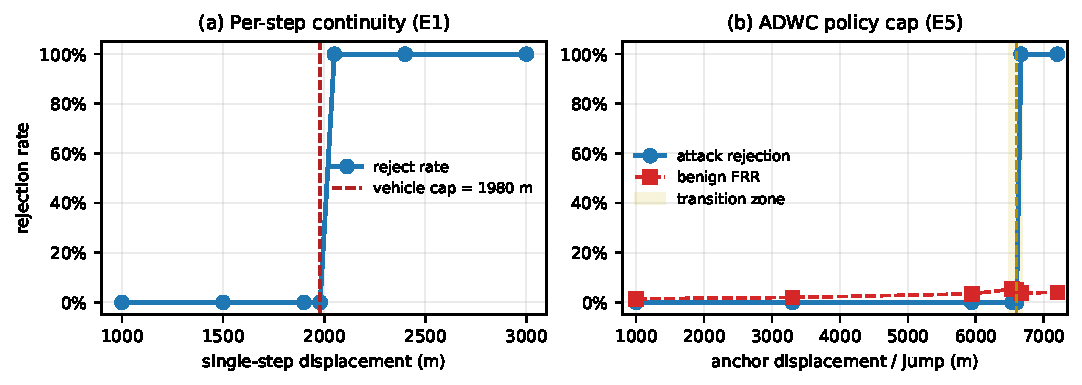
\includegraphics[width=\columnwidth]{fig_scurve}
  \caption{Two boundary S-curves. (a) Per-step continuity (E1):
  vehicle-tier proof generation accepts displacements up to
  $\tau_{\mathrm{vehicle}}\Delta t=\SI{1980}{m}$ and rejects larger
  displacements. (b) ADWC policy cap (E5). The existing T-Drive sweep
  tests $K{=}6$ anchor-distance continuity with
  $\mathrm{cap\_policy\_sq}=0.5\cdot\mathrm{tier\_anchor\_cap\_sq}$.   its transition near $\SI{6.6}{km}$ is a windowed ADWC boundary, not
  a per-step cap.}
  \label{fig:scurve}
\end{figure}

\subsection{Adversarial Reach Analysis}
\label{sec:eval-reach}

\textsc{TSIP} bounds an attacker's spatial influence per round to at most
$\tau_u\Delta t$ and per $K$-window to $\mathrm{cap}_{\mathrm{policy}}$. Under
the default vehicle profile, where $\tau_u\Delta t=\SI{1980}{m}$, one accepted
report can target at most $1{,}229$ cells, or about $12.3\%$ of the grid. Under
$K{=}6$ and $\mathrm{cap}_{\mathrm{policy}}=\SI{3.3}{km}$, the per-identity
per-window reach is at most $3{,}409$ cells, or $34.09\%$ of the grid.
Aggregate adversarial reach scales as $\rho\cdot34.09\%$. In the default 10\%
adversarial setting, worst-case pollution per $K$-window is at most $3.4\%$
before DP/SVT filtering.

\begin{proposition}[Bounded Adversarial Influence]
\label{prop:bounded-influence}
Let \(\rho\) be the malicious-client fraction in a reporting window,
\(a_{\mathrm{cap}}=A_{\mathrm{cap}}/|\mathcal{G}|\) be the fraction of grid
cells reachable under the public \(\mathrm{cap}_{\mathrm{policy}}\),
\(C_{\mathrm{clip}}\) be the per-report \(L_1\) clipping constant, and let
\(\alpha_{\mathrm{DP}}\in[0,1]\) denote the deployment-specific attenuation of
the released metric induced by the downstream thresholding/post-processing
pipeline. Then the expected released in-envelope bias attributable to accepted
malicious mass is bounded by
\[
\mathcal{B}_{\mathrm{rel}}
\le
\rho\cdot a_{\mathrm{cap}}\cdot C_{\mathrm{clip}}\cdot\alpha_{\mathrm{DP}}.
\]
For the default \(K{=}6\) policy, \(a_{\mathrm{cap}}\le 0.3409\), so
\[
\mathcal{B}_{\mathrm{rel}}
\le
0.3409\cdot\rho\cdot C_{\mathrm{clip}}\cdot\alpha_{\mathrm{DP}}.
\]
\end{proposition}
\begin{proof}[Proof sketch]
Each accepted malicious report is clipped to total count weight at most
\(C_{\mathrm{clip}}\), and its support is confined to the public reachable set
of size at most \(A_{\mathrm{cap}}\). At most a \(\rho\) fraction of accepted
clients are malicious in the window. Any downstream release pipeline can only
scale the observable contribution by its attenuation factor
\(\alpha_{\mathrm{DP}}\), yielding the stated product bound.
\end{proof}

\noindent\emph{Joint adaptive adversary.}

\textsc{TSIP} enforces an envelope, not ground truth. The following table
quantifies the size of that envelope and confirms that the envelope boundary is
the only remaining attack surface. A successfully verified in-envelope report
is \emph{accepted by design}, not a detection failure.

We evaluate a joint adaptive attacker that knows all public parameters and
jointly optimizes timing, mode tag, displacements, and payload to maximize
accepted malicious contribution. The setup uses $N{=}100$, 10\% malicious
clients, $T{=}50$, $K{=}6$, and
$\mathrm{cap}_{\mathrm{policy}}{=}\SI{3.3}{km}$.

Table~\ref{tab:joint-adaptive} shows two regimes. If the adversary decouples
the payload cell from the committed coordinate, payload binding rejects 98\%
of malicious cell-rounds with no in-envelope contributions admitted. If the
adversary instead keeps the payload consistent and stays inside the public
envelope, \textsc{TSIP} intentionally accepts the report (490/500 in-envelope
acceptance, by design). This is the residual risk bounded by
Proposition~\ref{prop:bounded-influence}, not an unrestricted bypass.
Consistently, the same payload-bound attack at $1.01{\times}$ the ADWC cap is
rejected in all 500 malicious cell-rounds. The coverage-cap column reports the
maximum reachable fraction of the $100{\times}100$ grid per malicious identity
per $K$-window under
$\mathrm{cap}_{\mathrm{policy}}=\SI{3.3}{km}$. At most 34.09\% per identity,
so even fully in-envelope attackers cannot pollute the entire heatmap. Aggregate
reach scales by the malicious-client fraction $\rho$.

\begin{table}[t]
\centering
\caption{Joint adaptive adversary results under the default $K{=}6$ policy.
The two 490/500 rows are distinct in-envelope optimizers with the same accepted
count but different cell spread and terminal offset.}
\label{tab:joint-adaptive}
\scriptsize
\setlength{\tabcolsep}{2pt}
\resizebox{\columnwidth}{!}{%
\begin{tabular}{llrrrrr}
\toprule
Pollution area / spatial influence & strategy & reject & accepted & in-envelope & terminal & coverage \\
         &          & rate   & cell-rds & adv. contribs & offset & cap/id \\
\midrule
0 cells & Random payload swap & 0.980 & 10/500  & 0/500   & \SI{0.00}{km} & 0\% \\
4 cells & Random valid payload & 0.894 & 53/500 & 43/500  & \SI{2.42}{km} & $\le$34.09\% \\
49 cells & Grid-search adaptive & in-envelope (by design) & 500/500 & 490/500 & \SI{6.62}{km} & $\le$34.09\% \\
2 cells & Mode/timing saturation & in-envelope (by design) & 500/500 & 490/500 & \SI{5.00}{km} & $\le$34.09\% \\
0 cells & $1.01{\times}$ ADWC boundary & 1.000 & 0/500 & 0/500 & \SI{3.33}{km} & 0\% \\
\bottomrule
\end{tabular}
}
\end{table}

\subsection{In-Envelope Poisoning and External-Layer Sensitivity}
\label{sec:eval-external-layer}

We therefore quantify the heatmap effect of a deployment-layer false-genesis attack and the
benefit of a transparent external gate. The simulator uses real pre-attack
traces to build per-user behavioral baselines, then has malicious users
promote a cold target cell. Without enrollment proof-of-location (PoL), the
attacker may choose a fake $c_0$ at the target. With verified genesis, the
trace must start at the real first location and move under the same per-step
envelope. A lightweight behavioral detector scores step-length and
heading-change histograms, distance-to-centroid, visited-cell entropy, and
activity bins, calibrated on benign validation windows at 1\% or 5\% target
FPR.

Table~\ref{tab:external-layer-combined} summarizes. Across cold-spot, hotspot, and corridor objectives, the external layer reduces accepted malicious mass by 90\%+ and eliminates false hotspot promotion across $\rho\in[0.01,0.30]$ with 1.2--3.2\% benign FRR.

\begin{table}[t]
\centering
\caption{Combined external-layer sensitivity and in-envelope poisoning results.
Panel~(a). Deployment-layer gap after the joint-adaptive test. Panel~(b):
pre-DP heatmap poisoning means over GeoLife/T-Drive and $K\in\{6,30\}$.}
\label{tab:external-layer-combined}
\scriptsize
\setlength{\tabcolsep}{2pt}
\resizebox{\columnwidth}{!}{%
\begin{tabular}{llrrrrr}
\toprule
\multicolumn{7}{c}{\textbf{(a) Deployment-layer gap}} \\
\midrule
Scenario & \textsc{TSIP} only & \textsc{TSIP}+ext. & Reduction & Benign FRR \\
GeoLife false-genesis (5\% FPR) & 360 & 0 & 100\% & 3.16\% \\
GeoLife false-genesis (1\% FPR) & 360 & 0 & 100\% & 0.79\% \\
T-Drive false-genesis (5\% FPR)  & 360 & 0 & 100\% & 7.19\% \\
Corridor acc.\ malicious mass    & 1.000 & 0.063 & 93.7\% & -- \\
Corridor pre-DP $L_1$ bias      & 0.1859 & 0.0077 & 95.9\% & -- \\
False hotspot probability & $>0$ at high $\rho$ & 0 & complete & 1.2--1.5\% \\
\midrule
\multicolumn{7}{c}{\textbf{(b) In-envelope heatmap poisoning}} \\
\midrule
Attack / Mode & Acc.\ mal. & $L_1$ bias & RMSE & Target lift & False HS@k & Jaccard \\
Cold, No int.\ & 1.000 & 0.1999 & 15.940 & 150.0 & 1.00 & 0.900 \\
Cold, \textsc{TSIP} & 1.000 & 0.0843 & 0.791 & 22.2 & 0.75 & 0.925 \\
Cold, \textsc{TSIP}+ext. & 0.578 & 0.0060 & 0.059 & 0.0 & 0.25 & 0.975 \\
Hotspot, No int.\ & 1.000 & 0.1799 & 13.418 & 135.0 & 1.00 & 0.900 \\
Hotspot, \textsc{TSIP} & 1.000 & 0.0866 & 0.763 & 22.0 & 0.50 & 0.950 \\
Hotspot, \textsc{TSIP}+ext. & 0.567 & 0.0053 & 0.057 & 0.0 & 0.25 & 0.975 \\
Corridor, No int.\ & 1.000 & 0.1899 & 4.623 & 0.0 & 1.00 & 0.900 \\
Corridor, \textsc{TSIP} & 1.000 & 0.1859 & 3.368 & 0.0 & 1.00 & 0.900 \\
Corridor, \textsc{TSIP}+ext. & 0.063 & 0.0077 & 0.223 & 0.0 & 0.00 & 1.000 \\
\bottomrule
\end{tabular}
}
\end{table}

Figure~\ref{fig:hotspot-pollution} sweeps the attacker fraction $\rho$ on a
harder target outside the benign top 20. With no integrity, $\rho\ge0.05$
consistently promotes a false hotspot into the top-20 set. \textsc{TSIP}-only
blocks the low-rate cases, but a sufficiently distributed in-envelope
pollution pattern still succeeds in 20\% of seeds at $\rho\in\{0.2,0.3\}$.
\textsc{TSIP}+external has zero false-hotspot events across all swept
$\rho$, with only 1.2--1.5\% benign false rejects. The omitted secondary
metrics follow the same ordering. No-integrity drives target-rank lift to
16.6--19.2 once $\rho\ge0.05$ and top-20 Jaccard falls to 0.60--0.69, whereas
\textsc{TSIP}+external keeps target-rank lift at 0 and Jaccard at 0.80.

\begin{figure}[t]
  \centering
  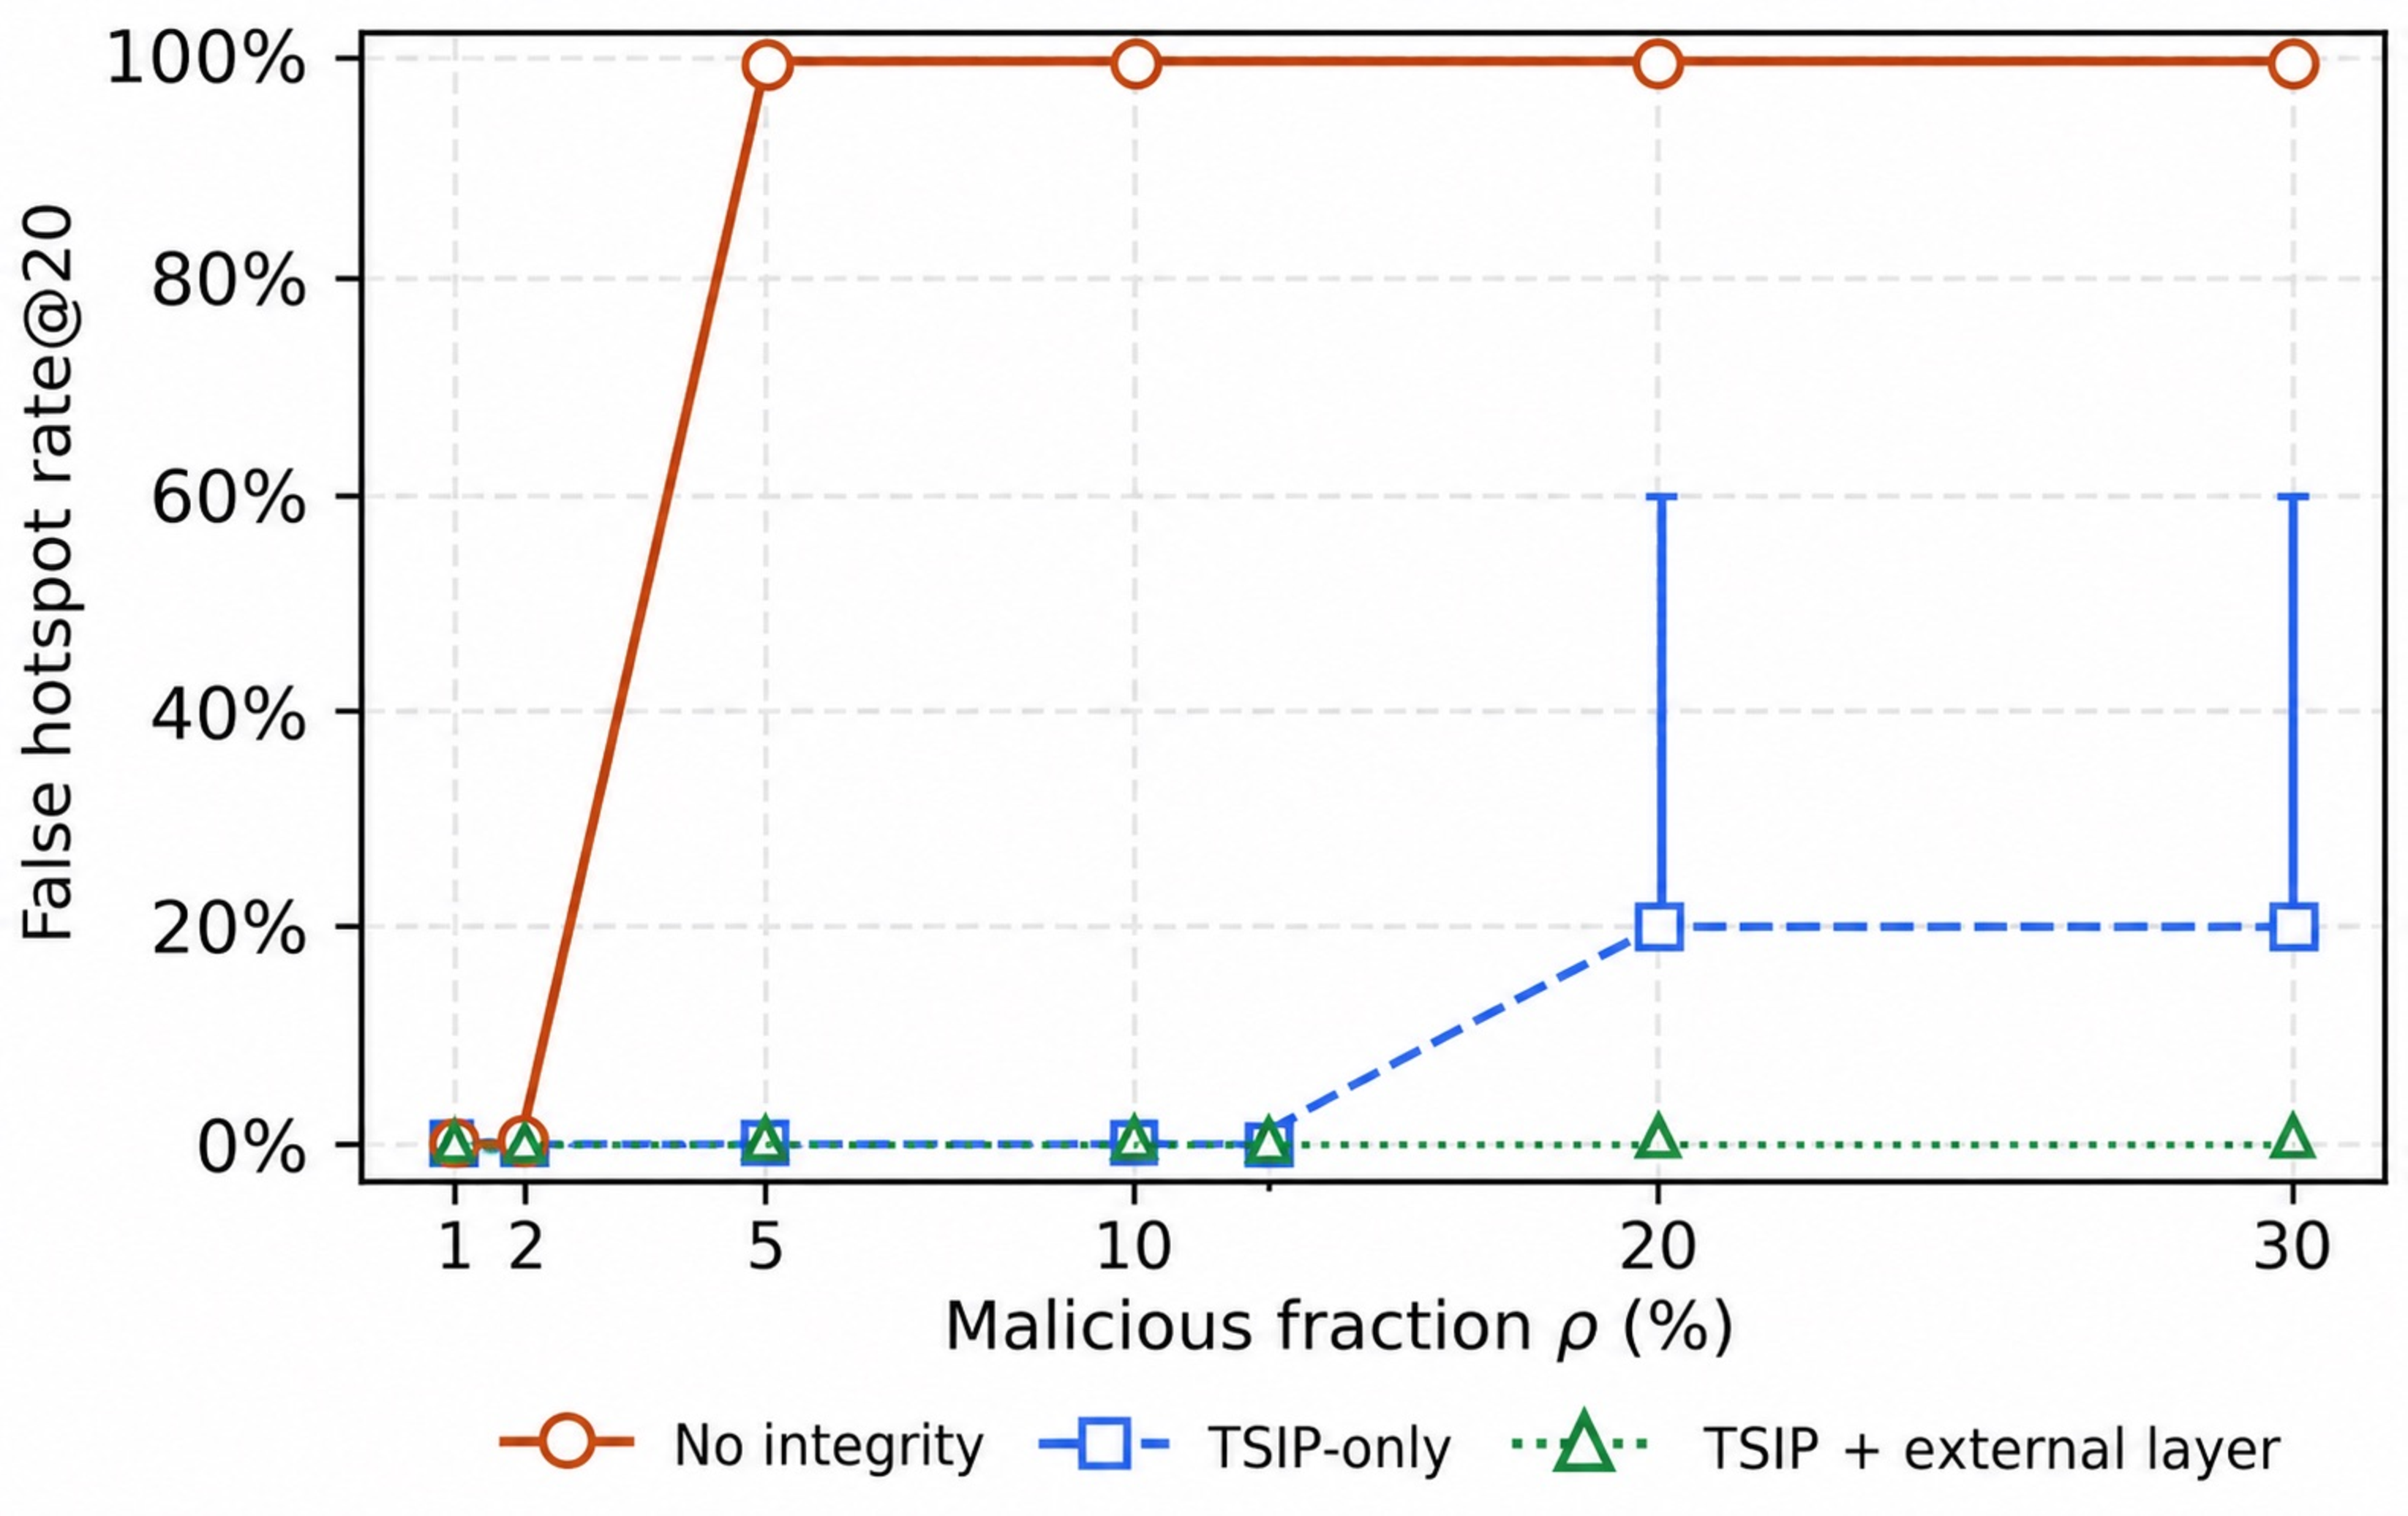
\includegraphics[width=\columnwidth]{fig_hotspot_pollution.pdf}
  \caption{Hotspot pollution sweep on GeoLife, reporting false top-20 hotspot
  probability across five seeds. The external layer eliminates false hotspot
  promotion across $\rho\in[0.01,0.30]$, while \textsc{TSIP}-only leaves a
  residual high-rate in-envelope surface.}
  \label{fig:hotspot-pollution}
\end{figure}

\subsection{Robustness and Privacy--Utility Across Datasets}
\label{sec:eval-robust}

Within-pipeline comparisons (Table~\ref{tab:ablation}) toggle only the ZK
components. Cross-mechanism comparisons assess qualitative ordering (see
\S\ref{sec:related-work} for the positioning table including Prio3 and RoFL analogues).
A DP $\varepsilon$ sweep on GeoLife confirms $\varepsilon$-invariance of
integrity ($\text{MRR}{=}1.00$ at every $\varepsilon$). The robust utility
rerun uses median/IQR over 10 released samples and reports RMSE/Pearson as the
headline statistics (Jaccard is unstable under small SVT threshold movements).
At $\varepsilon{=}1.0$ with 10\% A1 attackers, \textsc{TSIP-Full} yields
median RMSE~2.38 and Pearson~0.926 versus \textsc{No-Integrity}'s RMSE~2.25
and Pearson~0.954. A benign-only control (RMSE~5.67) confirms the
remaining degradation comes from session-gap/warmup withholding
rather than residual attacker mass. Full median/IQR and bootstrap CIs are in
Appendix~\ref{app:supp-results}.

\subsection{Scalability and Deployment Bottleneck}
\label{sec:eval-scale}

Population sweeps ($N\in\{50,200,500,1000\}$) show TPR stays at 1.00,
circuit-FRR remains 0, and pipeline FRR falls from $0.0402$ to $0.0002$ as
more cells clear the SVT threshold. Table~\ref{tab:cost-summary} consolidates
the two deployment profiles. Both use the same 3{,}056-constraint circuit,
128\,B proofs, and proving times well under the $\Delta t{=}\SI{60}{s}$
reporting window. On-device browser proving ($297$--$395$\,ms on iPhone and
Android) confirms the 1.5--1.6\,s host figure is dominated by software-path
overhead. A native ark-rs verifier sustains 3{,}320 proofs/s (16 workers,
3.01\,s for 10K proofs), corresponding to a steady-state capacity of
$\approx$199{,}000 simultaneously active clients at $\Delta t{=}\SI{60}{s}$.
Supporting tables are in Appendix~\ref{app:supp-results}.

\begin{table}[t]
\centering
\caption{Main cost summary for the evaluated \textsc{TSIPMain} implementation.}
\label{tab:cost-summary}
\scriptsize
\setlength{\tabcolsep}{3pt}
\begin{tabularx}{\columnwidth}{@{}Y >{\raggedleft\arraybackslash}p{2.2cm} >{\raggedleft\arraybackslash}p{2.2cm}@{}}
\toprule
Item & K6 & K30 \\
\midrule
Constraints & 3,056 & 3,056 \\
Public/private inputs & 14 / 23 & 14 / 23 \\
Proof size & 128\,B & 128\,B \\
snarkjs prover time & 1824.1\,ms & 1644.6\,ms \\
snarkjs verify & 1197.6\,ms & 1082.9\,ms \\
rapidsnark prover & 596.3\,ms & -- \\
Aggregator validation & $1.9\pm0.1$\,ms & same validator path \\
\bottomrule
\end{tabularx}
\end{table}

\subsection{ADWC Characterization of A3 Gradual Drift}
\label{sec:eval-a3}

A3 is evaluated as a \emph{parameterized ADWC defense}. Two deployment
profiles are used, $K{=}6$
($\mathrm{cap}_{\mathrm{policy}}{=}\SI{3.3}{km}$) and $K{=}30$
($\mathrm{cap}_{\mathrm{policy}}{=}\SI{16.5}{km}$). For $K{=}6$, TPR$=1.00$
across all five drift biases (0.20--1.00). For $K{=}30$, TPR ranges from 0.80
(bias$=0.20$) to 0.94 (bias$=0.40$), reflecting the larger window's softer
per-step resolution. $K{=}30$ is a stress test rather than the recommended
deployment. Tightening $\mathrm{cap}_{\mathrm{policy}}$ from $1.67\!\times$
to $0.67\!\times$ default raises $K{=}30$ TPR from 0.89 to 0.99
(Fig.~\ref{fig:adwc-policy-cap}, Appendix~\ref{app:supp-results}).

\begin{figure}[t]
  \centering
  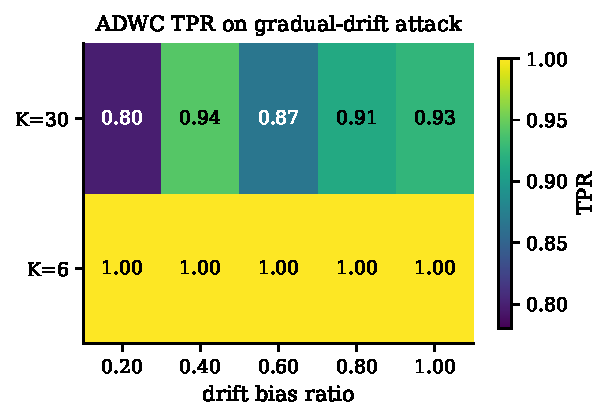
\includegraphics[width=\columnwidth]{fig_adwc_drift_k_heatmap.pdf}
  \caption{ADWC drift-rate $\times$ $K$-window TPR heatmap (GeoLife,
  vehicle tier, $\mathrm{cap\_policy}=0.5\!\times\!\mathrm{tier\_anchor\_cap}$,
  A3 gradual-drift at 10\% malicious rate). Each cell reports the
  current complete sweep aggregate for that $(K,\text{bias})$ pair.
  The short-window profile ($K{=}6$) achieves TPR~1.00
  across all tested drift biases. Longer windows allow more cumulative
  drift before the anchor check triggers.}
  \label{fig:adwc-drift-heatmap}
\end{figure}

\noindent\emph{$(\tau,\tau_2)$ sensitivity and session-gap baseline.}
\label{sec:eval-a3-session}
A $(\tau,\tau_2)$ sweep over $\{1,...,5\}^2$ (75 runs, 3 seeds per pair)
confirms DP-parameter invariance. Mean TPR~0.981 (range 0.951--1.000) and
session-withholding rate exactly 0.192 across all pairs (circuit-FRR~0),
since ZK verification precedes the DP/SVT release stage.
Under the production-default $G{=}\SI{30}{min}$ session-gap threshold, the
fraction of inter-window gaps exceeding $G$ is only $1.10\%$ (T-Drive) and
$2.12\%$ (GeoLife). At $G{=}\SI{60}{min}$ these fall to $0.76\%$ and $1.82\%$.

\section{Discussion and Limitations}
\label{sec:discussion}

\noindent\emph{Cryptographic scope and deployment requirements.}
The Trusted Computing Base (TCB) consists of the Groth16 setup, EA Ed25519
anchor keys, AEAD/channel authentication, and Poseidon/MiMC7 collision
resistance over BN254~\cite{shoup97}. If both Aggregators collude, input
privacy degrades to the public DP release while integrity still holds. False
genesis and A2b\label{sec:a2b} remain deployment-layer risks. They require
enrollment proof-of-location, device attestation, or behavioral risk scoring.
Operational dependencies include SRV-TS timing, warmup re-entry after session
gaps, and GPS-jitter margins in the speed caps. Client state is small
\(992\,\mathrm{B}\) at \(K{=}30\), but these policies determine the
honest-report loss discussed in \S\ref{sec:eval-robust}.

\section{Conclusion}
\label{sec:conclusion}

\textsc{TSIP} demonstrates that envelope-based cross-round trajectory
integrity can be enforced inside an ESA-style private aggregation pipeline
without exposing raw locations. The method adds a 128\,B Groth16 proof to each
submission and binds salted location commitments, identity commitment, ADWC
constraints, and same-primary payload binding inside one stateful circuit. The
prototype uses a 3{,}056-constraint hidden-primary circuit and keeps the
released heatmap under $\varepsilon_{\mathrm{total}}=1.0$ DP. Experiments on
T-Drive, GeoLife, and their stress subsets show that \textsc{TSIP} rejects the
modeled teleportation, credential-theft impersonation, replay,
proof-payload substitution, and gradual-drift attacks when they violate the
public envelope or the payload relation. Fully in-policy false trajectories are
accepted by design, but their spatial influence is bounded by the public
envelope and reduced further by downstream DP/SVT filtering. With a lightweight
behavioral external layer, false hotspot promotion is eliminated across all
tested adversarial fractions.

Future Work will extend \textsc{TSIP} in three directions. First, larger
combined-adversary sweeps are needed to cover more adaptive timing, mode, and
payload strategies. Second, stronger enrollment proof-of-location and
cross-device attestation policies should be evaluated because false genesis and
A2b remain deployment-layer risks. Third, a universal-setup proof-system port,
such as PLONK~\cite{Gabizon2019PLONK}, can remove the per-circuit ceremony and
make deployment easier. Societal-impact assessments of location integrity
systems~\cite{soderhall2025impact} should also guide production use.
\section*{Open Science}
\label{sec:open-science}
	We commit to NDSS Artifact Evaluation. The artifact will include Groth16 keys,
	Circom sources, Python microservices, a docker-compose harness,
	preprocessing scripts, and a small reproducible configuration ($N{=}10$,
	$T{=}3$). T-Drive and GeoLife are not redistributed, but source pointers and
	preprocessing instructions are provided. Upon acceptance and successful
	artifact evaluation, the artifact will be published with a permanent Zenodo DOI
	under a permissive license. The repository URL will be provided in the
	camera-ready version.

% conference papers do not normally have an appendix

% use section* for acknowledgment
\section*{Acknowledgment}
The use of generative AI tools was limited to grammar polishing
and figure caption refinement during manuscript preparation.
All technical content, system design, experimental methodology,
results, formal proofs, and analysis are the authors' own work.
The authors take full responsibility for all material in this paper.

\section*{Ethics Considerations}
\label{sec:ethics}
All evaluation traces come from public T-Drive and GeoLife releases. We do
not collect new human-subject data, contact data subjects, attempt
re-identification, or reproduce individual trajectories. The primary use case
is defensive integrity for public-interest heatmaps. Continuous location-proof
mechanisms are dual use, so any deployment would require an honest enrollment
authority and open circuit parameters. All adversarial and EA fault-injection
experiments use simulated clients against our own prototype, so no third-party
systems were probed.

\printbibliography

\appendices
\small

\section{Detailed Protocol}
\label{app:protocol}

\paragraph{Stage 3 aggregation.}
After Shuffler acceptance, each report is split into additive shares and
forwarded to two non-colluding aggregators, $A$ and $R$. Aggregator~A
receives $\mathsf{share}_A$ and Aggregator~R receives
$\mathsf{share}_R$, so neither party observes the plaintext contribution
alone. The Decoder reconstructs the aggregate, applies SVT threshold
filtering, adds Laplace perturbation, and releases the final DP heatmap.
Zero knowledge protects the proof layer, secure aggregation protects
intermediate inputs, and differential privacy protects the public output.

\paragraph{Re-enrollment policy.}
Warmup is enforced identically for first enrollment and re-enrollment.
Mode-only re-enrollment rotates \(\mathrm{mode\_tag}\), keeps
\(\mathrm{modeset\_commitment}\) unchanged, resets the epoch, and re-enters
warmup. Tier-changing re-enrollment may update
\(\mathrm{tier\_vmax\_sq}\) and recompute
\(\mathrm{modeset\_commitment}\). It also re-enters full warmup so no
immediately re-tiered submission enters the aggregate.

\paragraph{Session-timing filter.}
The squared step duration used by the circuit is Shuffler-issued rather than
client-chosen. Before proof generation, the client requests a timing token for
\((uid,\mathrm{epoch},w)\). The Shuffler stores
\(t_{\mathrm{last}}(uid)\), the server timestamp of the last accepted report,
selects a coarse current slot \(t_{\mathrm{slot}}\), and computes
\[
\Delta t=t_{\mathrm{slot}}-t_{\mathrm{last}}(uid).
\]
It rejects requests with \(\Delta t<\Delta t_{\min}\), and rejects or forces
warmup re-entry when \(\Delta t>G\). Otherwise it returns a signed timing token
containing
\[
(uid,\mathrm{epoch},w,t_{\mathrm{last}},t_{\mathrm{slot}},
\Delta t^2,\nu),
\]
where \(\nu\) is a nonce. The client proves against
\(\mathrm{step\_dt\_sq}=\Delta t^2\). On submission, the Shuffler verifies the
token signature, freshness, uid/epoch/round binding, nonce, and equality
between the token value and the proof public input. The production-style
defaults are \(\Delta t_{\min}=\SI{1}{s}\) and \(G=\SI{30}{min}\). The A3
characterization uses a stricter \(G{=}12\) minute setting to stress
sparse-trace behaviour and separate circuit-FRR, session-withholding, and
DP/SVT exclusion.

\paragraph{Salt management.}
The client stores \((\ell_w,r_w)\) with each accepted chain state. At round
\(w{+}1\), \(r_w\) is supplied as \(r_{\mathrm{prev}}\) to open the predecessor
hash, while the entry at index \(\max(0,w{+}1-K)\) supplies
\(r_{\mathrm{anchor}}\). Session reset does not reuse salts. The client starts
a new epoch, samples fresh salts, and retains the old ring only until all
pending anchor openings are no longer reachable.

\section{Circuit Constraints}
\label{app:circuit}

The circuit enforces the following constraints. C1--C20 cover trajectory,
state, identity, mode, ADWC, and hidden-cell encoding. C21 is the in-circuit
payload-binding relation.

\begin{table}[ht]
\centering
\caption{Circuit constraint summary. C1--C20 cover trajectory, state, identity,
mode, ADWC, and hidden-cell encoding. C21 is the in-circuit payload-binding
relation. All comparisons use LessEqThan(60) with Num2Bits range checks.}
\label{tab:constraint-summary}
\scriptsize
\setlength{\tabcolsep}{2pt}
\resizebox{\columnwidth}{!}{%
\begin{tabular}{@{}c p{3.2cm} p{4.4cm}@{}}
\toprule
\textbf{Group} & \textbf{Constraint} & \textbf{Purpose} \\
\midrule
C1--C3 &
\(\mathrm{Poseidon}(x_i,y_i,r)=\mathrm{hash}\) &
Bind salted location hashes for predecessor, current, and anchor \\
C4--C5 &
\(d^2\le\mathrm{tier\_vmax\_sq}\cdot\mathrm{step\_dt\_sq}\) \\
& \(d^2\le\mathrm{mode\_vmax\_sq}\cdot\mathrm{step\_dt\_sq}\) &
Per-step speed bounds under tier and selected mode \\
C6 &
\shortstack[l]{$\mathsf{Com}_{\mathsf{pri}} =$\\$\mathrm{Poseidon}(\mathrm{primary},$\\$\sigma_{\mathrm{pay}},r_{\mathrm{pri}})$} &
Commit hidden primary cell \\
C7 &
\shortstack[l]{$\mathrm{Poseidon}(\mathrm{secret},$\\$\mathrm{uid}_{field}) =$\\$\mathrm{secret\_commitment}$} &
Bind proof to registered per-user secret \\
C8--C10 &
\shortstack[l]{$\mathrm{Poseidon}(\mathrm{bitmap4},$\\$\mathrm{salt}) =$\\$\mathrm{modeset\_commitment}$} \\
& \(\mathrm{bitmap4[selected]}=1\) \\
& \shortstack[l]{$\mathrm{Poseidon}(\mathrm{selected\_mode},$\\$\mathrm{secret})=\mathrm{mode\_tag}$} &
Enforce hidden mode membership and tag consistency \\
C11--C13 &
\(\mathrm{anchor\_dist\_sq}\le\mathrm{tier\_anchor\_cap\_sq}\) \\
& \(\mathrm{anchor\_dist\_sq}\le\mathrm{cap\_policy\_sq}\) \\
& \(\mathrm{anchor\_dist\_sq}\le\mathrm{mode\_anchor\_cap\_sq}\) &
Conjunctive anchor-distance window caps \\
C14--C16 &
\(\mathrm{cap\_policy\_sq}\le\mathrm{tier\_anchor\_cap\_sq}\) \\
& \shortstack[l]{$\mathrm{tier\_anchor\_cap\_sq} =$\\$K^2\cdot\mathrm{tier\_vmax\_sq}$\\$\cdot\mathrm{step\_dt\_sq}$} \\
& \(\mathrm{mode\_vmax\_sq}\le\mathrm{tier\_vmax\_sq}\) &
Cap/tier consistency and mode bound enforcement. Fixed-slot reporting model. \\
C17--C20 &
\(x_2=q_x\cdot100+r_x,\,y_2=q_y\cdot100+r_y\) \\
& \(\mathrm{primary}=q_y\cdot100+q_x\) &
Derive hidden primary cell from hidden coordinate (100\,m grid) \\
C21 &
\shortstack[l]{$\mathsf{Com}_{A} =$\\$\mathrm{Poseidon}(\mathsf{Com}_{\mathsf{pri}},$\\$\mathsf{ctx},d_A,r_A)$} \\
& \shortstack[l]{$\mathsf{Com}_{R} =$\\$\mathrm{Poseidon}(\mathsf{Com}_{\mathsf{pri}},$\\$\mathsf{ctx},d_R,r_R)$} \\
& \shortstack[l]{$\mathsf{Com}_{\mathsf{pay}} =$\\$\mathrm{Poseidon}(\mathsf{Com}_{\mathsf{pri}},$\\$\mathsf{Com}_{A},\mathsf{Com}_{R},$\\$\mathsf{ctx},r_{\mathsf{pay}})$} &
In-circuit payload binding with the same hidden primary linked to all payload binders
under report context \(\mathsf{ctx}\). \(d_A,d_R\) are canonical digests of A/R
share contents. \\
\bottomrule
\end{tabular}%
}
\end{table}

The arity-3 Poseidon implementation with explicit integer checks compiles to
3{,}056 R1CS constraints in the evaluated circuit and keeps the Groth16 proof
size at 128\,B.

\subsection{Integer Semantics and Range Constraints}
\label{app:integer-semantics}

The BN254 scalar field does not provide a native integer ordering.
\textsc{TSIP} therefore treats every ordered value as a bounded integer before
using it in any comparison. Table~\ref{tab:integer-widths} lists the bit widths
enforced by the circuit or, for timestamps, by the Shuffler timing-token state
machine.

\begin{table}[ht]
\centering
\caption{Integer widths used by the \textsc{TSIP} circuit. All compared values
are below \(2^{60}\ll p_{\mathrm{BN254}}\approx2^{254}\).}
\label{tab:integer-widths}
\scriptsize
\begin{tabularx}{\columnwidth}{@{} l l X @{}}
\toprule
value & width & semantics \\
\midrule
\(x,y\) & signed 24-bit & shifted range check, about \(\pm8\)M meters \\
\(x_2-x_1,y_2-y_1\) & signed 25-bit & shifted difference check \\
\(\mathrm{step\_dt\_sq}\) & unsigned 24-bit & Shuffler-issued \(\Delta t^2\) \\
\(\mathrm{tier\_vmax\_sq}\) & unsigned 16-bit & enrollment tier speed cap squared \\
\(\mathrm{tier\_anchor\_cap\_sq}\) & unsigned 50-bit & public derived anchor cap \\
\(\mathrm{cap\_policy\_sq}\) & unsigned 50-bit & public policy anchor cap \\
\(d^2\) & unsigned 50-bit & per-step squared distance \\
\(\mathrm{anchor\_dist\_sq}\) & unsigned 50-bit & ADWC squared distance \\
\(t\) & unsigned 32-bit & server-side timing slot, not a circuit input \\
\bottomrule
\end{tabularx}
\end{table}

Signed coordinates are represented as field elements. For each coordinate
\(z\in\{x_1,y_1,x_2,y_2,x_a,y_a\}\), the circuit constrains
\(z+2^{23}\) with \(\operatorname{Num2Bits}(24)\), which accepts exactly
\(z\in[-2^{23},2^{23}-1]\) under the integer interpretation. Differences are
then formed in the field:
\[
dx=x_2-x_1,\qquad dy=y_2-y_1.
\]
The circuit constrains \(dx+2^{24}\) and \(dy+2^{24}\) with
\(\operatorname{Num2Bits}(25)\). Thus a negative field representative such as
\(p-\delta\) is accepted only when it corresponds to an integer
\(-\delta\) in the signed 25-bit range. The squared distances are computed as
\[
d^2=dx^2+dy^2,
\qquad
\mathrm{anchor\_dist\_sq}=(x_2-x_a)^2+(y_2-y_a)^2,
\]
and each result is constrained by \(\operatorname{Num2Bits}(50)\).

All public numeric inputs that can appear on the right-hand side of a bound
are range-checked before comparison. Let
\(\mathsf{N2B}_b(z)\) abbreviate \(\operatorname{Num2Bits}(b)(z)\):
\[
\mathsf{N2B}_{24}(\mathrm{step\_dt\_sq}),\quad
\mathsf{N2B}_{16}(\mathrm{tier\_vmax\_sq}),\quad
\mathsf{N2B}_{50}(\mathrm{tier\_anchor\_cap\_sq}),\quad
\mathsf{N2B}_{50}(\mathrm{cap\_policy\_sq}).
\]
This prevents a prover from setting, for example,
\(\mathrm{cap\_policy\_sq}\) close to \(p_{\mathrm{BN254}}\) and passing
\(\mathrm{anchor\_dist\_sq}\le\mathrm{cap\_policy\_sq}\) by field wraparound.

Every circuit inequality is implemented as
\(\operatorname{LessEqThan}(60)(a,b)=1\). The seven comparisons are the two
per-step caps, the three anchor-distance caps,
\(\mathrm{cap\_policy\_sq}\le\mathrm{tier\_anchor\_cap\_sq}\), and
\(\mathrm{mode\_vmax\_sq}\le\mathrm{tier\_vmax\_sq}\). Together, the
coordinate range checks, difference checks, distance/cap
\(\operatorname{Num2Bits}\) checks, seven \(\operatorname{LessEqThan}(60)\)
gadgets, the four C17--C20 quotient/remainder checks, and the C21
payload-binding subcircuit are included in the implementation's 3{,}056
constraints. The private-cell design binds the proof to
\(\mathsf{Com}_{\mathsf{pri}}\), \(\mathsf{Com}_{\mathsf{pay}}\),
\(\mathsf{Com}_{A}\), and \(\mathsf{Com}_{R}\) without exposing
\(\mathrm{primary}\) to the Shuffler. The Shuffler's
\(\mathrm{blob\_hash}\) check detects post-proof ciphertext-package
substitution but is not a plaintext-share commitment.

\subsection{Private-Payload Binding Tests}
\label{app:payload-binding-tests}

Table~\ref{tab:private-payload-binding} reports the functional binding tests
used for Experiment Group A. The implementation test harness exercises the
closed loop between Groth16 public inputs, hidden-cell encoding, in-circuit
payload binders, ciphertext forwarding, Shuffler transport checks, and
Aggregator-side format/context validation. A rejection in this table is
deterministic in the implemented harness. It is not a statistical detection
rate.

\begin{table*}[t]
\centering
\caption{Private-payload binding tests. Each negative case mutates one binding
surface after a valid baseline submission.}
\label{tab:private-payload-binding}
\scriptsize
\setlength{\tabcolsep}{3pt}
\begin{tabularx}{\textwidth}{@{}>{\raggedright\arraybackslash}p{0.30\textwidth}
>{\raggedright\arraybackslash}p{0.13\textwidth}
>{\raggedright\arraybackslash}p{0.21\textwidth}Y@{}}
\toprule
test & expected & attack surface & checked invariant \\
\midrule
Honest report with valid dense share blobs & accept & baseline functionality &
All C1--C21 constraints, Shuffler state checks, and Aggregator format/context
checks are jointly satisfiable. \\

Modify hidden-primary commitment public input & reject & proof/cell binder
tampering & C6 and C17--C20 bind the Groth16 proof to the hidden primary cell
derived from the hidden coordinate. \\

Modify report-level payload commitment & reject & payload binder tampering &
C21 binds the report-level payload commitment to the same hidden-primary
commitment and report context. \\

Modify A share-content commitment & reject & A-channel share binder tampering &
C21 binds the A-channel share-content commitment to the same hidden primary and
report context. \\

Modify R share-content commitment & reject & R-channel share binder tampering &
C21 binds the R-channel share-content commitment to the same hidden primary and
report context. \\

Modify \(\mathrm{blob\_hash}\) public input & reject at Shuffler transport
check & ciphertext-package tampering & The Shuffler recomputes
\(\mathrm{blob\_hash}\) from the uploaded ciphertext package before forwarding. \\

Replace A ciphertext after proof & reject at Shuffler transport check &
post-proof ciphertext malleability & The Shuffler recomputes
\(\mathrm{blob\_hash}\) from the uploaded ciphertext package before forwarding. \\

Replace R ciphertext after proof & reject at Shuffler transport check &
post-proof ciphertext malleability & The same \(\mathrm{blob\_hash}\)
recomputation rejects post-proof substitution on the R channel. \\

Swap A share from another report & reject & cross-report share mix-and-match &
C21 context binding and Shuffler \(\mathrm{blob\_hash}\) recomputation prevent
transplanting one report's A blob into another report. \\

Swap R share from another report & reject & cross-report share mix-and-match &
C21 context binding and Shuffler \(\mathrm{blob\_hash}\) recomputation prevent
transplanting one report's R blob into another report. \\

Replay old share blob with fresh proof & reject & replay / stale payload reuse &
Payload binders, \(\mathrm{blob\_hash}\), and context binding tie the package
to the current uid, epoch, round, and aggregation context. \\

Malformed dense/VDAF share blob & reject by Aggregator validation &
plaintext share format & Decryption, channel, domain, length, and dense-share
format checks reject malformed blobs even if the route envelope is
syntactically present. \\

Wrong primary witness for coordinate & proof generation or verification fails &
hidden-cell encoding bypass & C17--C20 require
\(\mathrm{primary}=100q_y+q_x\) derived from the hidden coordinate. \\

Valid proof but A/R channel labels swapped & reject & channel confusion &
Aggregator A and R decrypt with channel-specific labels, so swapped labels fail
before aggregation. \\

Same proof with different ciphertext blob & reject & proof reuse with new
payload & Ciphertext replacement changes \(\mathrm{blob\_hash}\) and breaks the
transport integrity check before forwarding. \\

Changed context/window\_id/uid/epoch in share commitment & reject &
context binding & The payload binders and \(\mathrm{blob\_hash}\) are derived
from report context, so context edits break the proof/payload relation. \\
\bottomrule
\end{tabularx}
\end{table*}

\section{Per-Attack Defense Analysis}
\label{app:attacks}

\begin{lemma}[End-to-end payload binding]
\label{lem:e2e-payload}
Assume Groth16 knowledge soundness, binding/collision resistance of the
commitment relations, Shuffler ciphertext-package authenticity, and
Aggregator-side format/context validation. If a submission is accepted, then
except with negligible probability the payload binders accepted by the
Shuffler are bound to the same hidden primary cell opened in the
\textsc{TSIPMain} witness, and the forwarded ciphertext package matches the
reported transport digest.
\end{lemma}

\begin{proof}
C17--C20 force the witness primary cell to equal
\(100\lfloor y_i/100\rfloor+\lfloor x_i/100\rfloor\) for the hidden current
coordinate. C6 binds this primary to the hidden-primary commitment.
C21 binds the same hidden-primary commitment to the report-level payload
commitment and the A/R share-content commitments under the current report
context. The Shuffler accepts only ciphertext packages whose digest matches
\(\mathrm{blob\_hash}\), and AEAD/context checks prevent replacing those blobs
under another \(uid\), epoch, round, or channel. After decryption, each
Aggregator accepts only dense-share material that passes length, domain,
redundancy, and format checks. Therefore a successful proof-payload
substitution would require a Groth16 extraction failure, a
Poseidon/commitment collision, an undetected ciphertext-package substitution,
or an Aggregator-side validation failure.
\end{proof}

\paragraph{A1--A5 coverage by Theorem~\ref{thm:traj-integrity}.}
A1 (teleportation) is covered by C4/C5 per-step tier and mode speed caps
($d>\tau_u\Delta t$ fails verification). A2a (credential-theft impersonation) is
covered by C7 secret binding and Shuffler chain-state continuity. A3 (gradual
drift) is bounded by C11--C15 ADWC with conjunctive tier, policy, and mode
anchor caps. A4 (Sybil collusion) relies on threshold EA attestation (CA3).
A5 (replay) is prevented by the Shuffler's per-\((uid,w)\) chain-state machine
that rejects reused predecessors. A2b (credential/device transfer) is outside
\textsc{TSIP}'s cryptographic guarantee and is addressed by deployment-layer
mitigations discussed in \S\ref{sec:discussion}.

\paragraph{A6 proof-payload substitution.}
\label{app:a6}
Under Groth16 knowledge soundness, an accepting proof implies a witness
satisfying C1--C21. Table~\ref{tab:private-payload-binding} separates the A6
payload-binding cases by attack surface. Forged hidden-primary or payload
binder inputs, ciphertext replacement after proof generation, A/R channel
confusion, cross-report share swaps, stale-share replay, malformed dense/VDAF
blobs, and changed uid/epoch/window context. All negative cases are rejected
by proof verification, Shuffler transport checks, or Aggregator-side
format/context validation.

\section{Game-Based Proofs}
\label{app:proofs}

\subsection*{D.0 Full Integrity Game Hops}

Let \(\mathsf{Win}\) denote the event that a PPT adversary \(\mathcal{A}\)
outputs an accepting submission whose extracted witness violates at least one
of E1--E6.

\textit{Game \(G_0\):}
Real \textsc{TSIP} acceptance game.
\[
\Pr[\mathsf{Win}_0]=\mathsf{Adv}^{\mathsf{int}}_{\mathcal{A}}.
\]

\textit{Game \(G_1\):}
Abort if the Groth16 knowledge-soundness extractor fails on any of the
\(\le q\) accepting proofs. By knowledge soundness and a union bound,
\[
|\Pr[\mathsf{Win}_1]-\Pr[\mathsf{Win}_0]|
\le
q\cdot\mathsf{Adv}^{\mathsf{KS\text{-}Groth16}}.
\]
In \(G_1\), every accepted submission has an extracted witness satisfying the
circuit relation.

\textit{Game \(G_2\):}
Abort if any two distinct openings collide under Poseidon. Across the location
commitments, hidden-primary commitment, report-level payload commitment, A/R
share-content commitments, secret commitment, and modeset commitment, for a
constant \(c_{\mathsf{P}}\) openings per report,
\[
|\Pr[\mathsf{Win}_2]-\Pr[\mathsf{Win}_1]|
\le
c_{\mathsf{P}}q\cdot\mathsf{Adv}^{\mathsf{CR\text{-}Poseidon}}.
\]

\textit{Game \(G_3\):}
Abort if any two distinct chain-state preimages collide under MiMC7:
\[
|\Pr[\mathsf{Win}_3]-\Pr[\mathsf{Win}_2]|
\le
q\cdot\mathsf{Adv}^{\mathsf{CR\text{-}MiMC7}}.
\]

\textit{Game \(G_4\):}
Abort if an accepted ciphertext/blob package violates commitment binding or
ciphertext-package authenticity:
\[
\begin{aligned}
|\Pr[\mathsf{Win}_4]-\Pr[\mathsf{Win}_3]|
&\le
q\cdot\mathsf{Adv}^{\mathsf{BIND\text{-}Commit}} \\
&\quad {}+
q\cdot\mathsf{Adv}^{\mathsf{AUTH\text{-}Blob}}
+
\mathrm{negl}(\lambda).
\end{aligned}
\]

In \(G_4\), each accepted submission has a unique witness satisfying the
circuit relation and a unique chain-state preimage. Under SRV-TS, C4/C5 imply
E1. The Shuffler state machine implies E4. And C11--C15 imply E5. The
hidden-primary derivation (C17--C20, C21) and secret binding (C7) are
absorbed into Lemma~\ref{lem:same-primary} and Lemma~\ref{lem:e2e-payload}
respectively. Hence
\(\Pr[\mathsf{Win}_4]=0\), and summing the hop bounds gives
Theorem~\ref{thm:traj-integrity}. The payload-binding hops are summarized
separately in Theorem~\ref{thm:payload-binding}.

\subsection*{D.1 Full G2 Experiment}

Let \(\mathcal{A}\) be a PPT adversary corrupting a strict subset
\(S\subset\{\mathsf{Shuffler},\mathsf{AggregatorA},\mathsf{AggregatorR},
\mathsf{EA}\}\) such that
\[
\bigl(|S\cap\{\mathsf{AggregatorA},\mathsf{AggregatorR}\}|\le1
\wedge
\mathsf{EA}\notin S\bigr)
\vee
S\subseteq\{\mathsf{EA}\}.
\]
For bit \(b\in\{0,1\}\), define
\(\mathsf{Exp}^{\mathsf{priv}}_{\mathsf{TSIP},\mathcal{A}}(\lambda,b)\) as
follows.

\begin{enumerate}
\item \(\mathcal{A}\) outputs two equal-length trajectory sets \(T_0,T_1\) for
an honest user \(u^\star\). Both trajectories must use the same public
non-location metadata and induce the same per-step and ADWC predicate outcomes,
including the same accept/reject sequence under the public caps. This
restriction matches the scope of G2. Chain topology, submission timing, and
accept/reject signals are public control metadata and are outside the
coordinate-hiding target. The derived primary cell is not public metadata. G2
does not claim trajectory-shape unlinkability.

\item The challenger runs \textsc{TSIP} on \(T_b\) using fresh salts, sharing
randomness, encryption randomness, and proof randomness.

\item \(\mathcal{A}\) receives the joint view of all corrupted servers in \(S\)
across all rounds and outputs \(b'\in\{0,1\}\).
\end{enumerate}

The experiment returns \(b'\). \textsc{TSIP} satisfies G2 if, for every such
\(\mathcal{A}\),
\[
\begin{aligned}
&\left|
\Pr[\mathsf{Exp}^{\mathsf{priv}}_{\mathsf{TSIP},\mathcal{A}}(\lambda,0)=1]
-
\Pr[\mathsf{Exp}^{\mathsf{priv}}_{\mathsf{TSIP},\mathcal{A}}(\lambda,1)=1]
\right| \\
&\qquad\le \mathrm{negl}(\lambda).
\end{aligned}
\]

\subsection*{D.2 Hybrid Argument for G2}

We prove the bound
\begin{equation}
\label{eq:g2-bound}
\begin{aligned}
\Delta_{\mathsf{priv}}
&:=
\left|
\Pr[\mathsf{Exp}^{\mathsf{priv}}=1\mid b=0]
-
\Pr[\mathsf{Exp}^{\mathsf{priv}}=1\mid b=1]
\right| \\
&\le
n\cdot\mathsf{Adv}^{\mathsf{ZK\text{-}Groth16}} \\
&\quad {}+
c_{\mathsf{H}}n\cdot\mathsf{Adv}^{\mathsf{HIDE\text{-}Poseidon}} \\
&\quad {}+
n\cdot\mathsf{Adv}^{\mathsf{IND\text{-}CPA/AEAD}} \\
&\quad {}+
n\cdot\mathsf{Adv}^{\mathsf{IndexHide\text{-}Share}} \\
&\quad {}+
\mathrm{negl}(\lambda),
\end{aligned}
\end{equation}
where \(c_{\mathsf{H}}\) is the constant number of salted Poseidon commitments
whose messages are hidden in the privacy hybrid.

\textit{\(H_0\):}
Real game with \(b=0\).

\textit{\(H_1\) (Shuffler proof view):}
Replace each Groth16 proof \(\pi_t\) with a simulated proof
\(\tilde{\pi}_t\leftarrow\mathsf{Sim}(\mathsf{vk},x_t)\). This simulation
covers the entire \textsc{TSIPMain} witness, including the trajectory witness,
hidden-cell witness, and payload-binding witness. The Shuffler still sees
public tier/mode tags, chain topology, submission timing, public binders, and
accept/reject outcomes. These are fixed leakage in G2's challenge. By
\(\mathsf{ZK\text{-}Groth16}\),
\[
|\Pr[H_1]-\Pr[H_0]|
\le
n\cdot\mathsf{Adv}^{\mathsf{ZK\text{-}Groth16}}.
\]

\textit{\(H_2\) (Shuffler commitment view):}
Replace each location commitment and payload binder with a salted Poseidon
commitment to a uniformly random message under fresh salts. By
\(\mathsf{HIDE\text{-}Poseidon}\), applied to a constant number
\(c_{\mathsf{H}}\) of hiding commitments per round,
\[
|\Pr[H_2]-\Pr[H_1]|
\le
c_{\mathsf{H}}n\cdot\mathsf{Adv}^{\mathsf{HIDE\text{-}Poseidon}}.
\]

\textit{\(H_3\) (Shuffler ciphertext view):}
Replace each routed ciphertext package with an AEAD encryption of a dummy
fixed-layout blob of the same public length. By AEAD confidentiality,
\[
|\Pr[H_3]-\Pr[H_2]|
\le
n\cdot\mathsf{Adv}^{\mathsf{IND\text{-}CPA/AEAD}}.
\]

\textit{\(H_{4-6}\) (Aggregator, Decoder, and EA views):}
If Aggregator A (resp.\ R) is corrupted, replace its plaintext-share view with
the single-Aggregator index-hiding simulator (\(n\cdot\mathsf{Adv}^{\mathsf{IndexHide\text{-}Share}}\)
per view). The threat model excludes simultaneous corruption of both
Aggregators. The Decoder sees only reconstructed aggregate counts before
SVT/Laplace release, which is pure \(\varepsilon_{\mathrm{total}}\)-DP and
independent of the coordinate choice. The EA view contains only enrollment
metadata \((\mathsf{uid},\mathsf{com}_{\mathsf{sec}},\mathsf{com}_{\mathsf{modeset}},
\mathsf{tier\_vmax\_sq},\mathsf{exp},\mathsf{kid},\sigma)\), independent of
\(T_b\) by construction.

In \(H_6\), all non-leakage values visible to any admissible corrupted set are
independent of \(b\). Mirroring the chain from \(b=1\) connects the two real
games with total advantage bounded as claimed.

\textit{Leakage acknowledged.}
A corrupted Shuffler observes
\[
\mathsf{hash}_{\mathsf{curr},t}
=
\mathsf{hash}_{\mathsf{prev},t+1}
\]
and per-\(uid\) submission timing. G2 protects coordinate and primary-cell
confidentiality, not unlinkability. This is an intentional trust-boundary
choice. \qed

\subsection*{D.3 Concrete Budget Instantiation}

Under the default $(t{=}3,n{=}5)$ configuration, suppose each anchor
attestation costs $C_{\mathrm{anchor}}\approx\$0.50$ (e.g., a CAPTCHA-backed
rate-limited enrollment check) and a vehicle-tier VC issuance costs
$c_{\mathrm{VC}}(\mathrm{vehicle})\approx\$5.00$ (e.g., a one-time Know Your
Customer verification or a proof-of-insurance deposit). An adversary with
budget $B=\$10{,}000$ can therefore sustain at most
$m\le\lfloor 10000/(3\cdot 0.50+5.00)\rfloor=1538$
simultaneously active Sybil identities, each spatially bounded to
$\le 34.09\%$ of the grid per $K$-window. At the minimum tier (walk, assuming
negligible VC cost), the bound tightens to
$m\le\lfloor 10000/1.50\rfloor=6666$. These bounds are economic, not
cryptographic, but they demonstrate that \textsc{TSIP} raises the per-identity
attack cost from near-zero account creation to a quantifiable external budget
constraint.

\emph{Tier soundness.}
Acceptance requires each attestation to verify against its declared
\(\mathsf{kid}\) public key and at least \(t\) distinct valid signatures over
the same enrollment tuple. Forging a different accepted tier without
corresponding keys implies signature forgery or verifier failure.

\emph{VC cost and bounded Sybil.}
Each accepted enrollment binds one credential-backed tier assignment, so
identities cannot be lifted to higher tiers without corresponding credential
issuance. Under CA3, each accepted Sybil identity requires at least \(t\)
valid anchor signatures. Combining the per-anchor acquisition cost with the
credential cost yields the budget bound in Theorem~\ref{thm:bounded-sybil}.

\section{Supplementary Results}
\label{app:supp-results}
\enlargethispage{3\baselineskip}

Integrity is \(\varepsilon\)-invariant in the GeoLife sweep
(\(\mathrm{MRR}=1.00\) for \textsc{TSIP-Full}). Sparse released-set Jaccard is
reported as a supplemental metric because it is dominated by threshold
crossings. The \((\tau,\tau_2)\) sweep confirms that proof verification is
DP-parameter invariant (mean TPR \(=0.981\), circuit-FRR \(=0\)), and session
withholding is timing-driven rather than ADWC-driven. Randomized attack sweeps
use three seeds. The robust GeoLife utility table uses 10 released samples with
user-level bootstrap CIs. Datasets cover dense and sparse regimes, and A1--A6
are representative rather than exhaustive. Tables and the figure below provide
the numeric details cited in the main evaluation.

\begin{figure}[t]
\centering
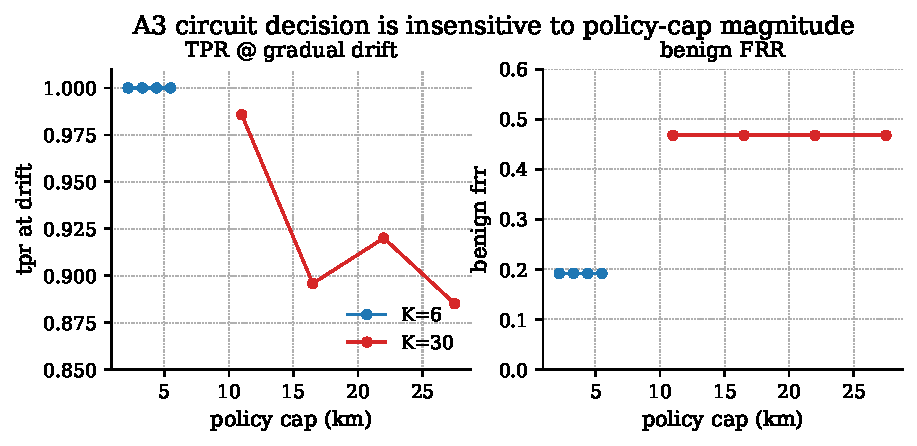
\includegraphics[width=\columnwidth]{fig_adwc_policy_cap.pdf}
\caption{Policy-cap sensitivity sweep (GeoLife, \(K{=}30\) long-window stress
setting, vehicle tier, 10\% malicious A3 adversary). Tightening
\(\mathrm{cap\_policy}\) from \(1.67{\times}\) to \(0.67{\times}\) default
raises TPR from 0.89 to 0.99. Session-withholding rate (dashed) is flat at
\(\approx0.47\) regardless of cap value, confirming that the ADWC predicate
rejects no honest trace.}
\label{fig:adwc-policy-cap}
\end{figure}

\begin{table}[t]
\centering
\caption{Robust GeoLife utility rerun at \(\varepsilon{=}1.0\). Both rows
use 10\% A1 attackers and report median with IQR over 10 released
samples.}
\label{tab:exact-jaccard-ablation}
\scriptsize
\setlength{\tabcolsep}{2pt}
\resizebox{\columnwidth}{!}{%
\begin{tabular}{lrrrrrr}
\toprule
mode & MRR & FRR & Jaccard med. & Jaccard IQR & RMSE med. (IQR) & Pearson med. (IQR) \\
\midrule
\textsc{TSIP-Full} & 1.0000 & 0.1068 & 0.5000 & 0.3750--1.0000 & 2.3784 (2.2885--2.4320) & 0.9262 (0.7229--0.9488) \\
\textsc{No-Integrity} & 0.0000 & 0.0000 & 1.0000 & 1.0000--1.0000 & 2.2499 (2.2013--2.2719) & 0.9544 (0.9544--0.9638) \\
\bottomrule
\end{tabular}}
\end{table}

\begin{table}[!b]
\centering
\caption{Payload-size breakdown across four wire-format layers.}
\label{tab:combined-supp}
\scriptsize
\setlength{\tabcolsep}{3pt}
\begin{tabularx}{\columnwidth}{@{}l r X@{}}
\toprule
\multicolumn{3}{c}{\textbf{(a) Payload-size breakdown}} \\
\midrule
layer & bytes & contents \\
\midrule
L1 proof object & 128 & compressed BN254 Groth16 tuple
\((A,C\in\mathbb{G}_1, B\in\mathbb{G}_2)\) \\
L1 public scalars & 448 & evaluated public-input vector
(field-element encoding) \\
L2 proof JSON & 806--807 & snarkjs proof.json with decimal coordinates,
curve/protocol tags, and JSON punctuation \\
L2 public JSON & 862 & snarkjs public.json for the same public signals \\
L3 integrity pkg. & \(\approx2{,}100\) & proof object + public inputs +
chain metadata + authentication fields \\
L4 full frame & 5{,}694 & L3 plus encrypted additive-share envelopes and
prototype metadata \\
\bottomrule
\end{tabularx}
\end{table}

\begin{table}[!b]
\centering
\caption{Native ark-rs verifier throughput scaling for 10{,}000 \(K{=}6\)
proofs on the evaluation host. Throughput is near-linear through 8 workers and
remains sufficient for the \(\SI{60}{s}\) reporting window at every measured
worker count.}
\label{tab:verifier-throughput}
\scriptsize
\setlength{\tabcolsep}{3pt}
\begin{tabular}{@{}r r r r@{}}
\toprule
workers & wall time (s) & QPS & effective ms/proof \\
\midrule
1  & 15.7101 & 636.53  & 1.5710 \\
4  &  4.5123 & 2216.16 & 0.4512 \\
16 &  3.0123 & 3319.70 & 0.3012 \\
\bottomrule
\end{tabular}
\end{table}

\FloatBarrier
\end{document}
